\chapter{Resultaten}
% TODO: Bespreek waarom het goed of slecht is, wat de sterke en zwakke kanten zijn.
De validatie van de NLP-profielen gebeurt aan de hand van een neuraal netwerk zoals beschreven in \autoref{sub:chapt4_evaluatie_profielen}. Deze basisimplementatie voor het neuraal netwerk bleek niet krachtig genoeg om verbanden te vinden in de inputdata, en voorspelt in de meeste gevallen gewoon 4 van de 5 sterren. Daarom besloten we om eerst de basisimplementatie van het neuraal netwerk bij te schaven, zodat de vergelijking van NLP-profielen zinvol is. Concreet hebben we de optimizer en learning rate van het basismodel vervangen van (SGD, $0.01$) naar (ADAGRAD, $0.0002$). Alle resultaten uit \autoref{sub:chapt5_nlp_resultaten} maken gebruik van deze aangepaste implementatie.\newline
\autoref{fig:chapt5_inleiding_sgd_suckt_combined} toont dat SGD niet geschikt is voor dit optimalisatieprobleem. Deze conclusie geldt voor iedere combinatie van inputprofielen. Het onderzoek naar een betere optimizer staat volledig beschreven in \autoref{sec:chapt5_neuraal_netwerk}.

\begin{figure}[H]
    \begin{subfigure}{.5\textwidth}
        \centering
        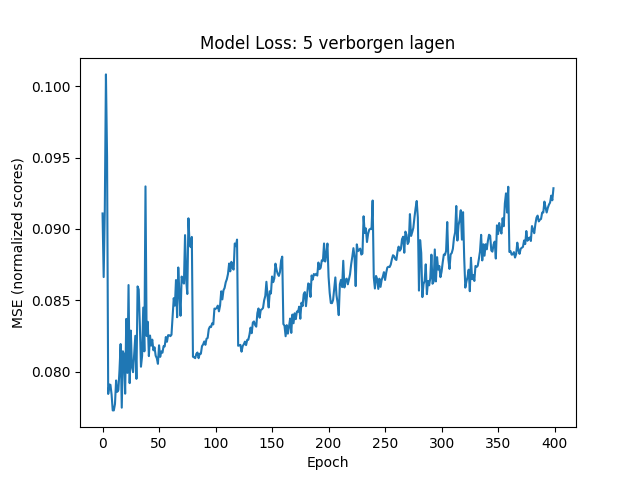
\includegraphics[width=1\linewidth]{fig/chapt5/inleiding/mlp5_2023-05-19_13h32__EPOCHS=400_LOSS=0.0929_LR=0.01.png}
        \caption{SGD, learning rate = $0.01$}
        \label{fig:chapt5_inleiding_sgd_suckt_1}
    \end{subfigure}
    \begin{subfigure}{.5\textwidth}
        \centering
        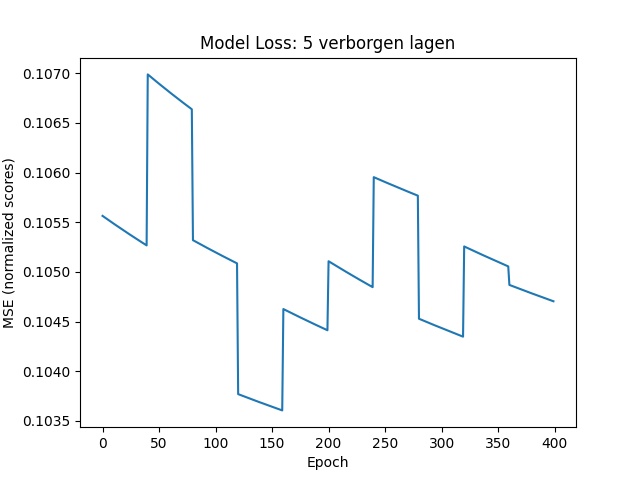
\includegraphics[width=1\linewidth]{fig/chapt5/inleiding/mlp5_2023-05-19_13h32__EPOCHS=400_LOSS=0.105_LR=0.0001.png}
        \caption{SGD, learning rate = $0.0001$}
        \label{fig:chapt5_inleiding_sgd_suckt_2}
    \end{subfigure}
    \caption{Neurale netwerken getraind met dezelfde inputdata}
    \label{fig:chapt5_inleiding_sgd_suckt_combined}
\end{figure}


% TODO: resultaten met grafieken en bespreking waarom (vermoedelijk) iets beter of slechter scoort
\section{NLP-profielen}
\label{sub:chapt5_nlp_resultaten}
De eerste stap is het valideren van gebruikers- en restaurantprofielen gegenereerd door verschillende combinaties van parameters. We bekijken welke combinatie het neuraal netwerk het beste in staat stelt om accurate voorspellingen te maken. Vervolgens analyseren we of de gebruikte BERTopic modellen overeenkomen met de resultaten van de clusteringsmetrieken uit \autoref{sub:chapt4_eval_clustering}.

% TODO LEGENDE VOOR MODELNAMEN?
% standaard of indien aangegeven

% TODO betere titel?
\subsection{Parameters voor gebruikers- en restaurantprofielen}
\label{sub:chapt5_vergelijking_profielen}
Het eerste experiment is de prestaties vergelijken van een offline BERTopic model tegenover zijn online variant. Hiervoor gebruiken we voor beide modellen dezelfde parameterconfiguratie, het enige verschil is dat het offline model op 2\% van de data getraind is terwijl de online variant de volledige dataset gebruikt. % todo welke modellen hebben we gebruikt?

% offline vs ONLINE
\mijnfiguur[H]{width=10cm}{fig/chapt5/NLP/nlp_comparison_offline.png}{Vergelijken van profielen zonder sentiment analysis gegenereerd door een offline model van 50 topics tegenover online modellen van 50 en 400 topics.}{fig:chapt5_nlp_offline_vs_online}

Uit \autoref{fig:chapt5_nlp_offline_vs_online} kunnen we concluderen dat het gebruik van een online model een significante verbetering geeft. Daarom gaan we vanaf hier enkel de online modellen met elkaar vergelijken. Een andere onderzoeksparameter is het gebruik van sentiment analysis, hierbij onderzoeken we het effect van sentiment analysis op gebruikers- en restaurantprofielen. Verder analyseren we ook of eenzelfde trend tussen een gebruikersprofiel en een restaurantprofiel zichtbaar is.

% USER - RESTAURANT (sentiment) \label{fig:chapt5_nlp_sentiment_comparison}
% A: vergelijk (kolom 2 VS 6) \label{fig:chapt5_nlp_sentiment_user}   
% B: vergelijk (rij 3 VS 6) \label{fig:chapt5_nlp_sentiment_restaurant}
\begin{figure}[H]

        \centering
        \parbox[b]{0.6\textwidth}{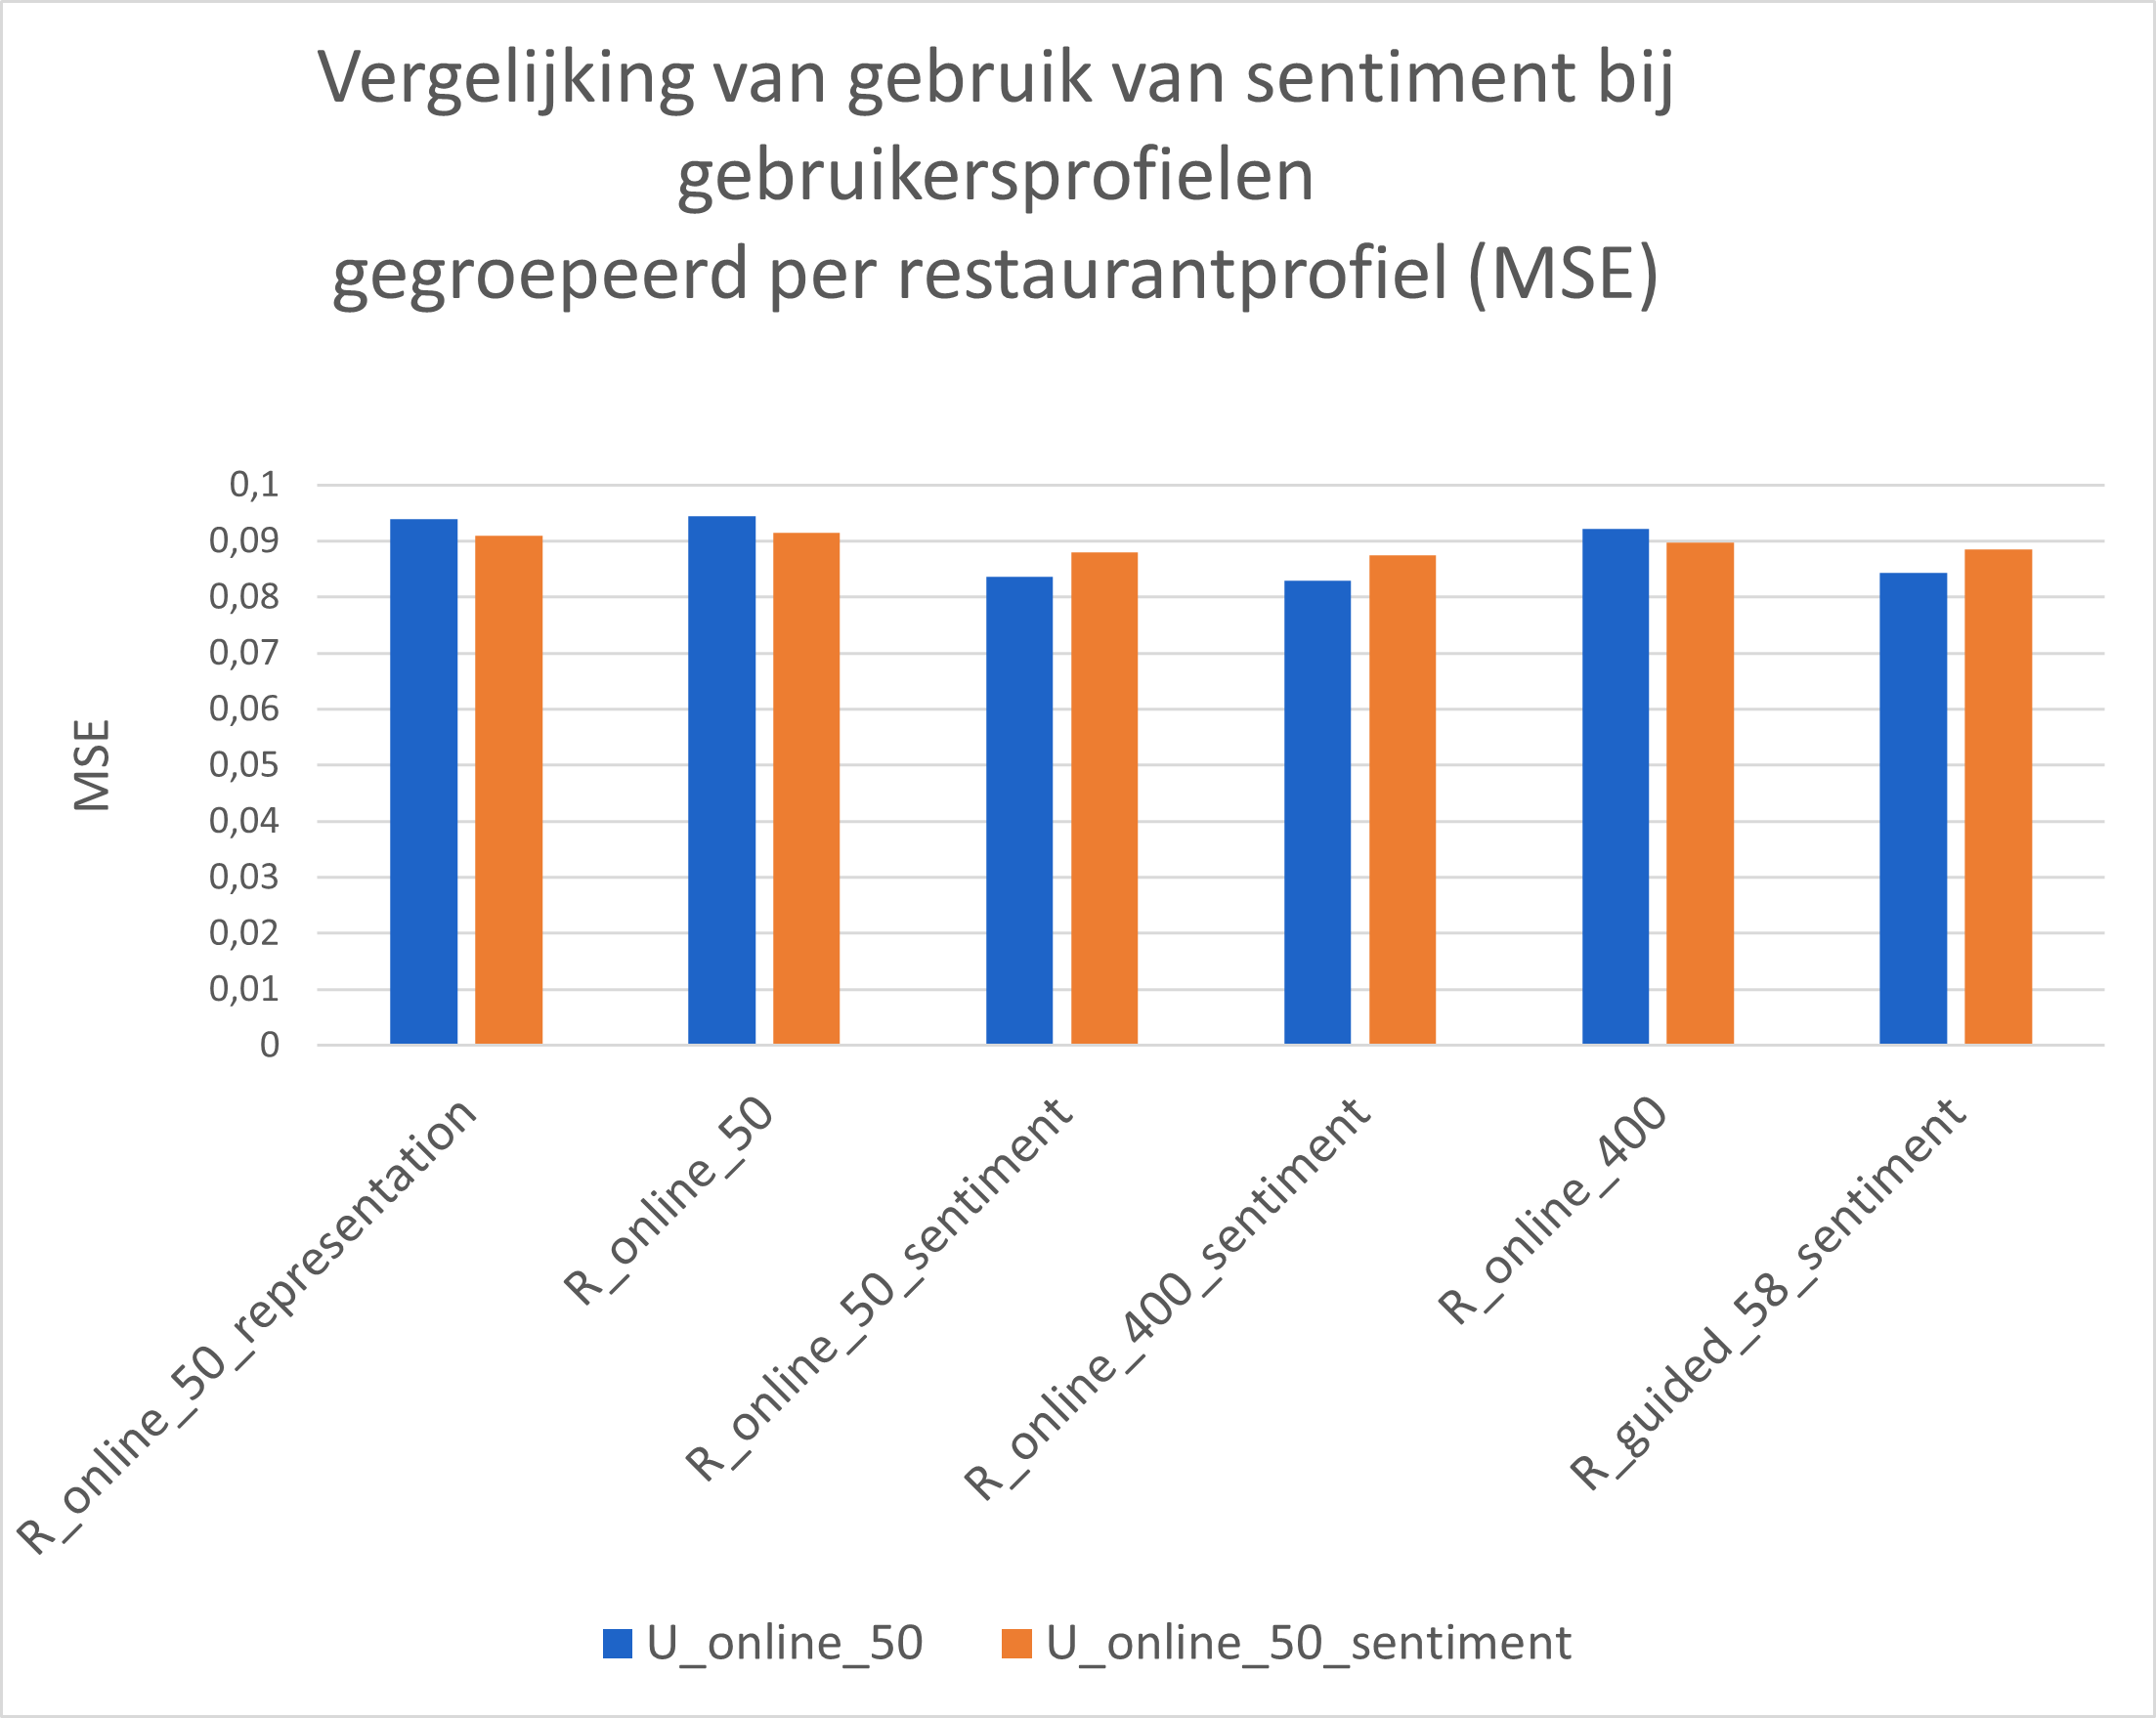
\includegraphics[width=\linewidth]{fig/chapt5/NLP/nlp_comparison_sentiment_gebruiker.png}}\quad
        \parbox[b]{0.37\textwidth}{
        \subcaption{Gebruikersprofiel zonder sentiment (blauw) en gebruikersprofiel met sentiment (oranje) vergeleken met verschillende restaurantprofielen op basis van MSE.}\label{fig:chapt5_nlp_sentiment_user}}
        \\[.5cm]

        \centering
        \parbox[b]{0.6\textwidth}{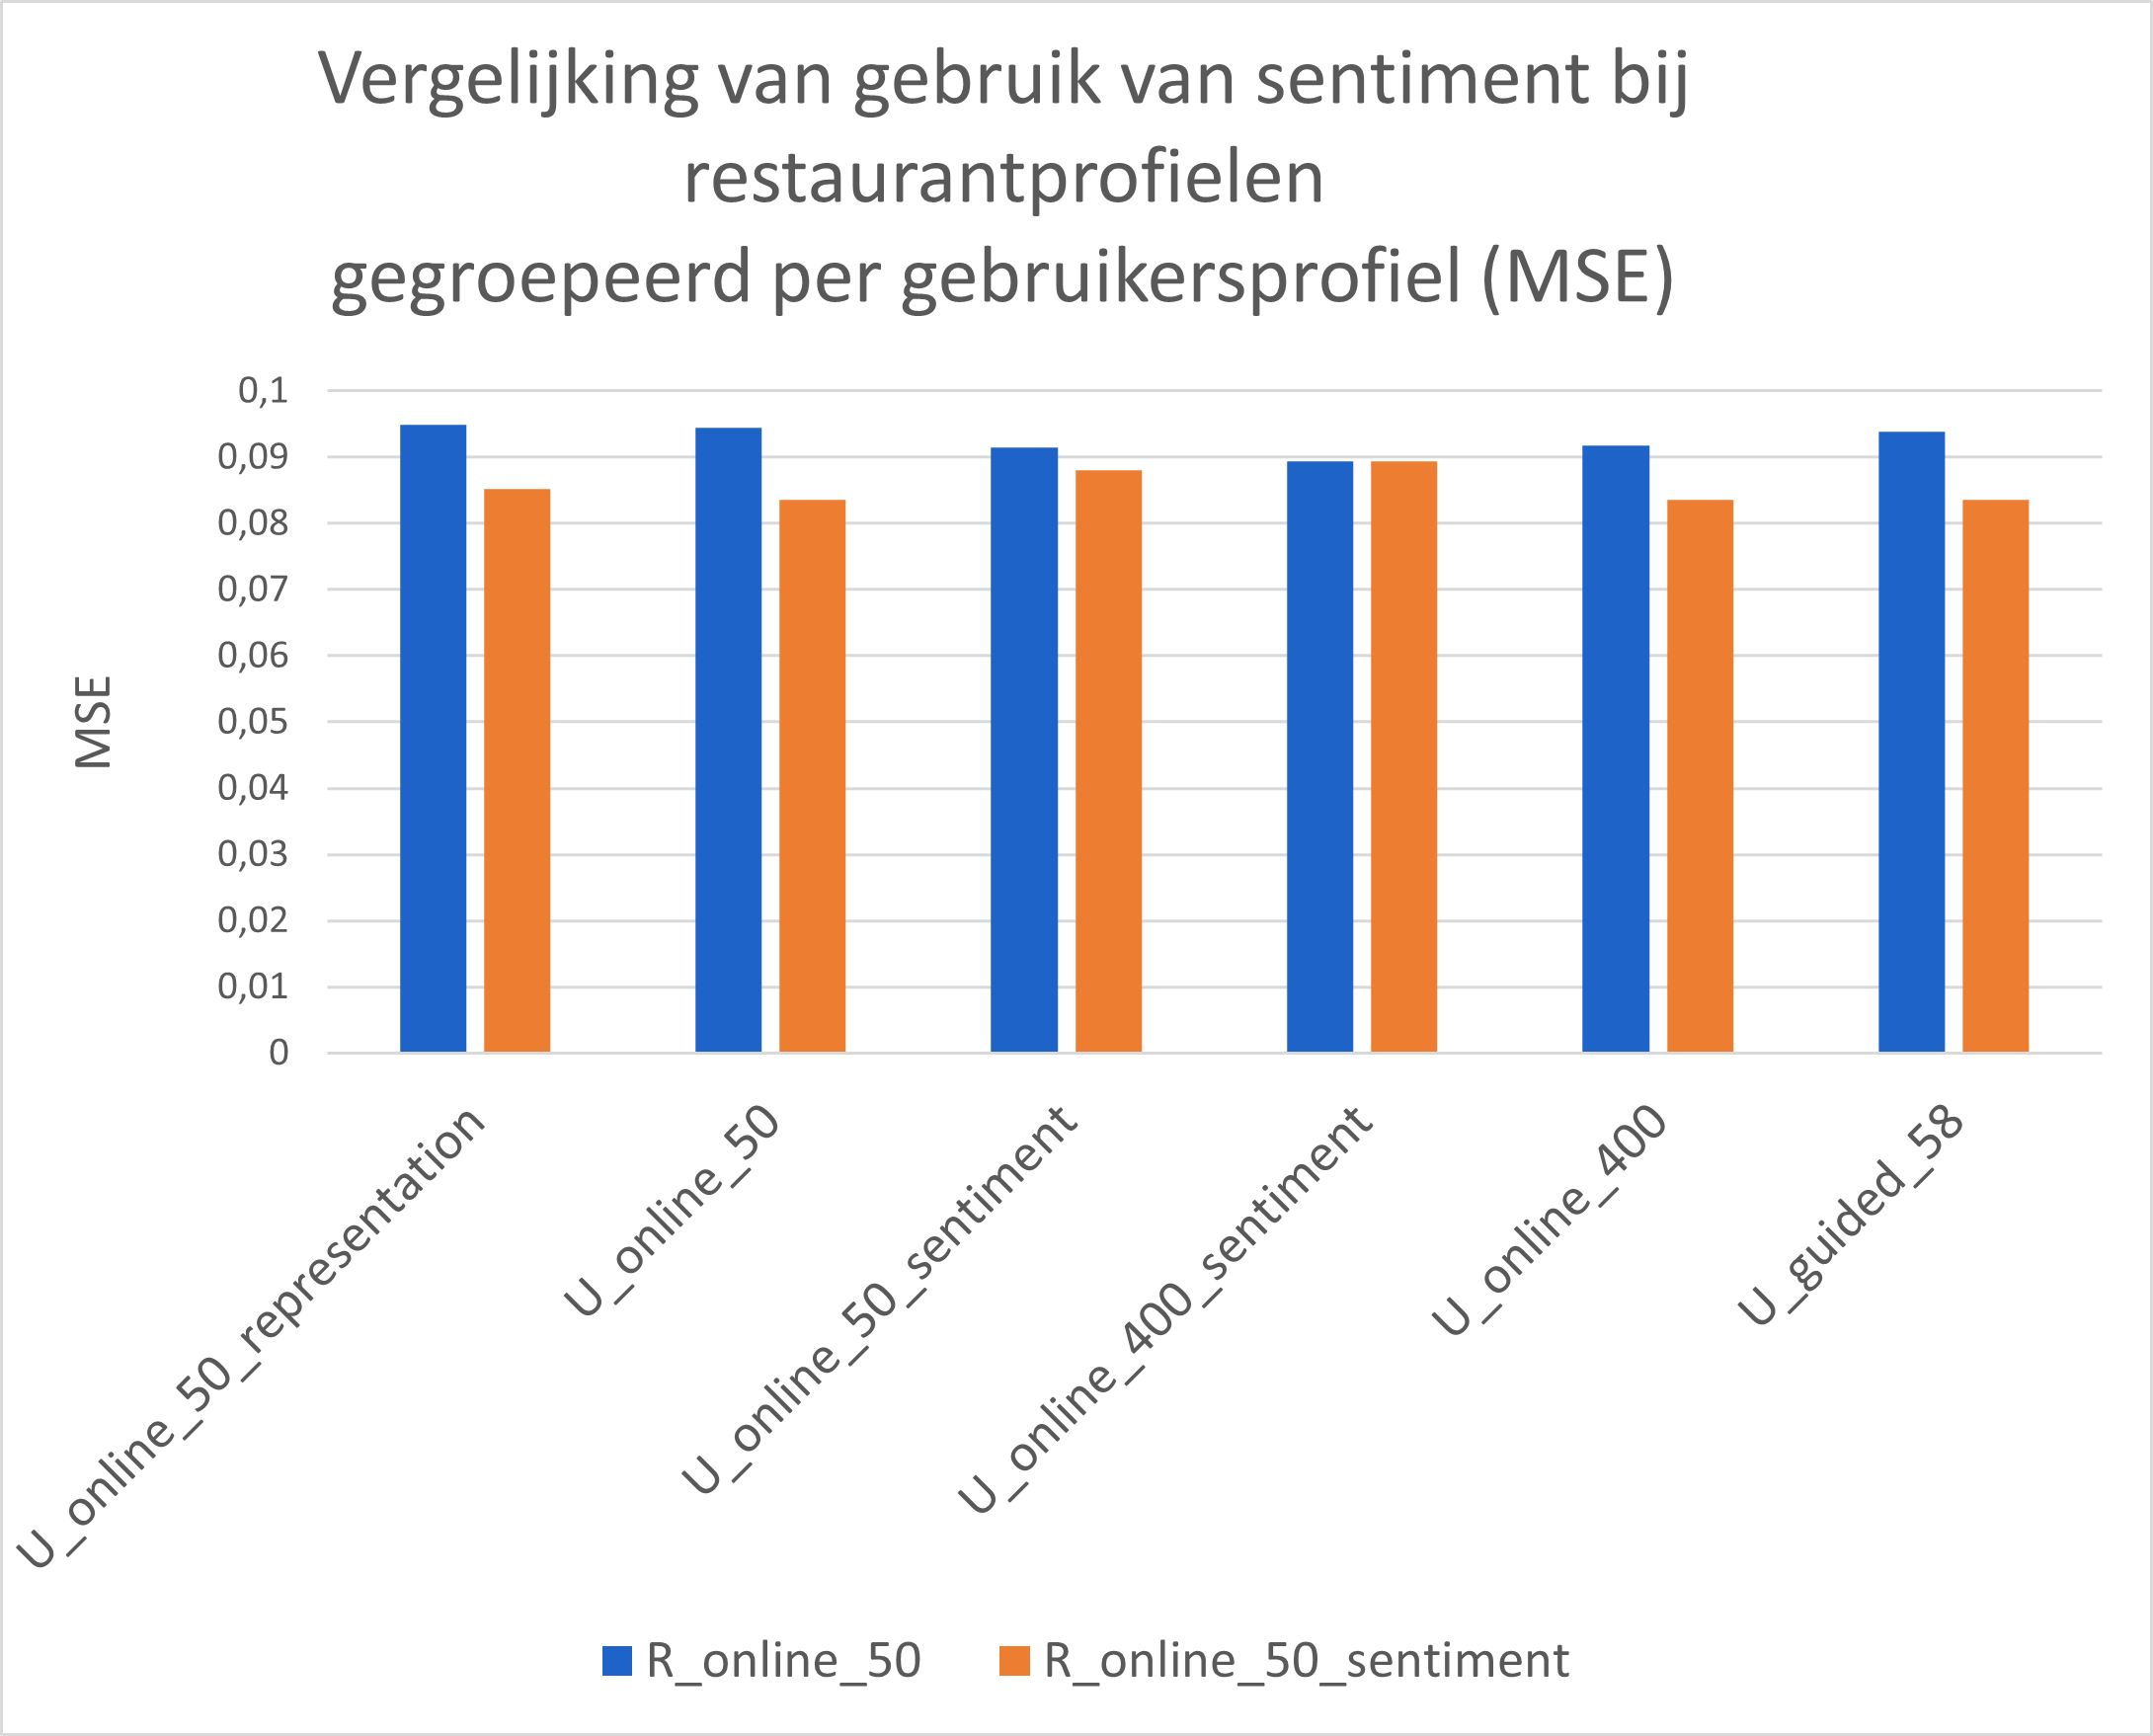
\includegraphics[width=\linewidth]{fig/chapt5/NLP/nlp_comparison_sentiment_restaurant.png}}\quad
        \parbox[b]{0.37\textwidth}{
        \subcaption{Restaurantprofiel zonder sentiment (blauw) en restaurantprofiel met sentiment (oranje) vergeleken met verschillende gebruikersprofielen op basis van MSE.}\label{fig:chapt5_nlp_sentiment_restaurant}}
        \\[.5cm]

        \caption{Analyse van de toegevoegde waarde van sentiment analysis bij het genereren van gebruikers- en restaurantprofielen.}
        \label{fig:chapt5_nlp_sentiment_comparison}
\end{figure}

Uit de grafieken afgebeeld in \autoref{fig:chapt5_nlp_sentiment_comparison} kunnen we enkele zaken besluiten. Het toevoegen van sentiment analysis bij gebruikersprofielen resulteert in een kleine stijging in performantie indien de restaurantprofielen geen sentiment gebruiken. Indien een restaurantprofiel wel sentiment gebruikt presteert een gebruikersprofiel zonder sentiment beter zoals in \autoref{fig:chapt5_nlp_sentiment_user}. Analoog kunnen we de vergelijking maken voor restaurantprofielen. In dit geval zien we een gelijkaardig effect. Aan de hand van \autoref{fig:chapt5_nlp_sentiment_restaurant} nemen we waar dat er een significante daling is in MSE bij het gebruik van sentiment bij restaurantprofielen in combinatie met gebruikersprofielen zonder sentiment. Indien een gebruikersprofiel toch sentiment toevoegt is deze stijging in performantie merkbaar kleiner.

Voor de beste prestaties gaan we enkel sentiment gebruiken bij een restaurantprofiel, dit kunnen we afleiden uit beide grafieken door de combinatie van profielen met de laagste MSE te nemen. De hypothese uit \autoref{sub:chapt4_users_vs_restaurants} waarbij we geen sentiment analysis gaan toepassen op de gebruikersprofielen maar wel op de restaurantprofielen is dus geldig. \\

% TODO \label{fig:chapt5_nlp_approx_vs_topics} 
% A: vergelijk (kolom 2 VS 1) telkens approx vs geen approx => analoog: vrij gelijkaardig voor user      \label{fig:chapt5_nlp_approx_vs_topics_users}
% B: vergelijk (rij 2 VS 1) telkens approx vs geen approx => vrij gelijkaardig voor restaurants          \label{fig:chapt5_nlp_approx_vs_topics_restaurant}
\begin{figure}[H]

        \centering
        \parbox[b]{0.6\textwidth}{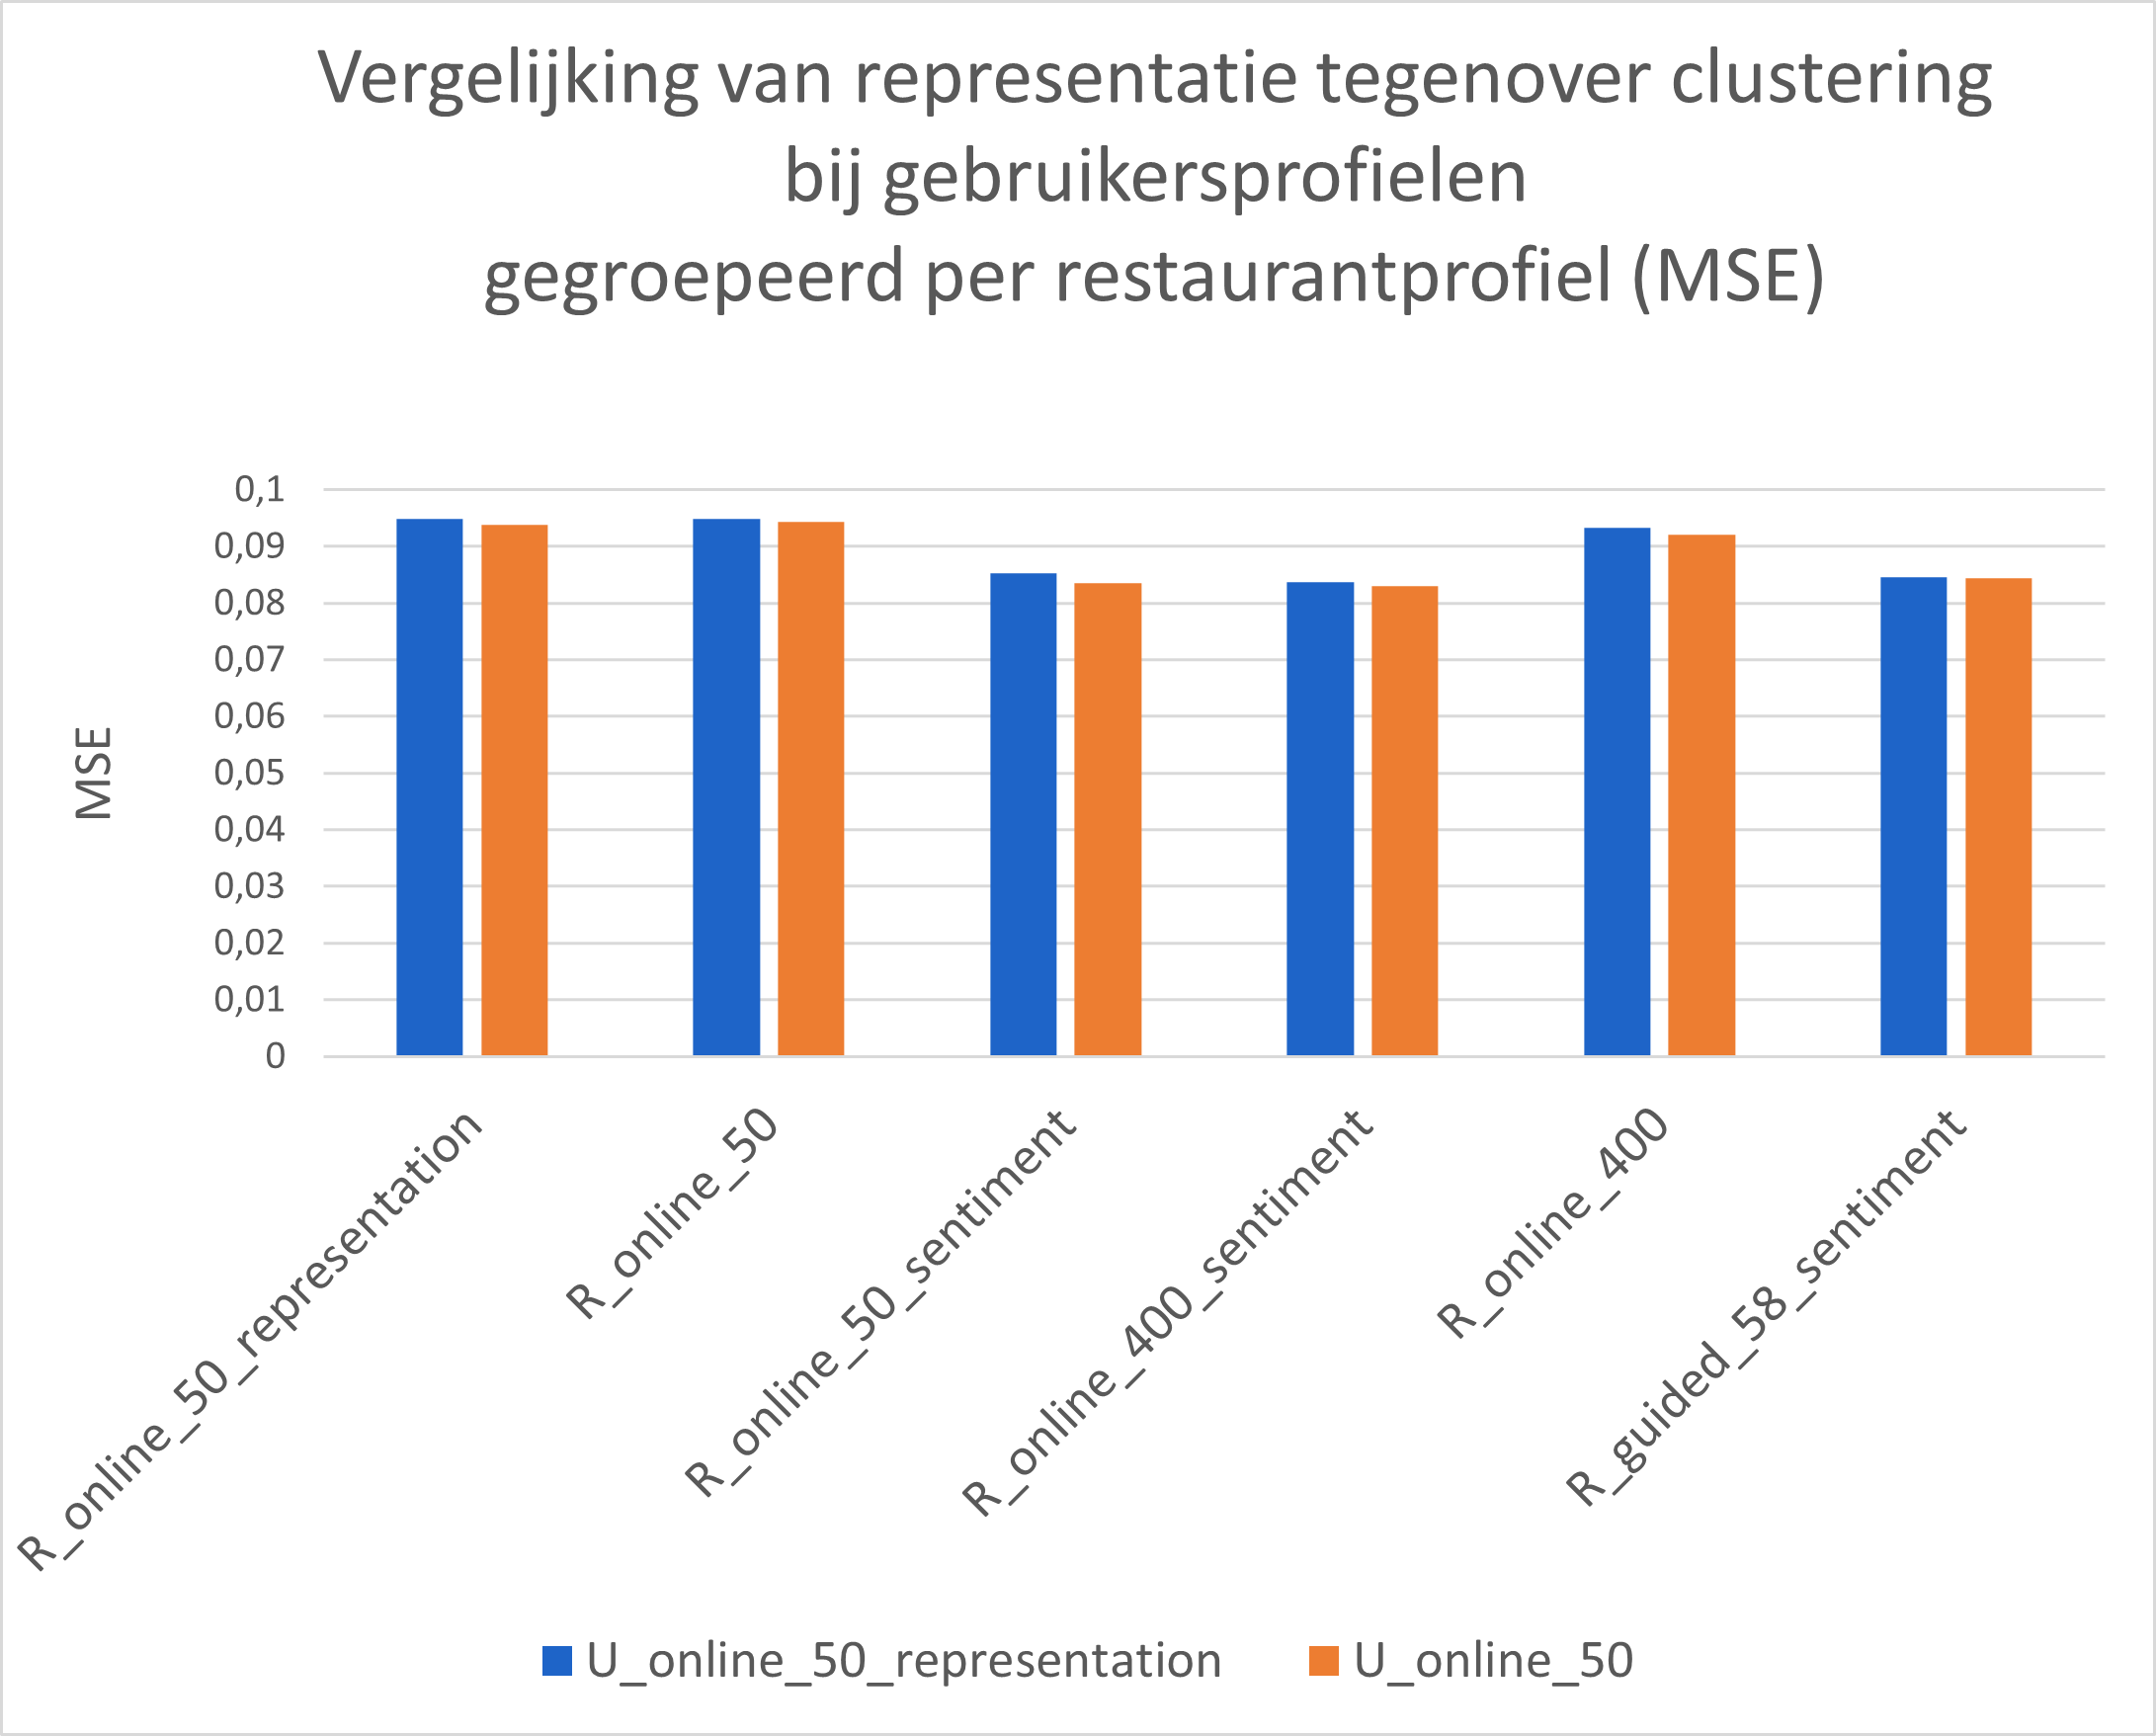
\includegraphics[width=\linewidth]{fig/chapt5/NLP/nlp_comparison_approx_gebruiker.png}}\quad
        \parbox[b]{0.37\textwidth}{
        \subcaption{Gebruikersprofiel op basis van representatie (blauw) en gebruikersprofiel op basis van clustering (oranje) vergeleken met verschillende restaurantprofielen op basis van MSE.}\label{fig:chapt5_nlp_approx_vs_topics_users}}
        \\[.5cm]

        \centering
        \parbox[b]{0.6\textwidth}{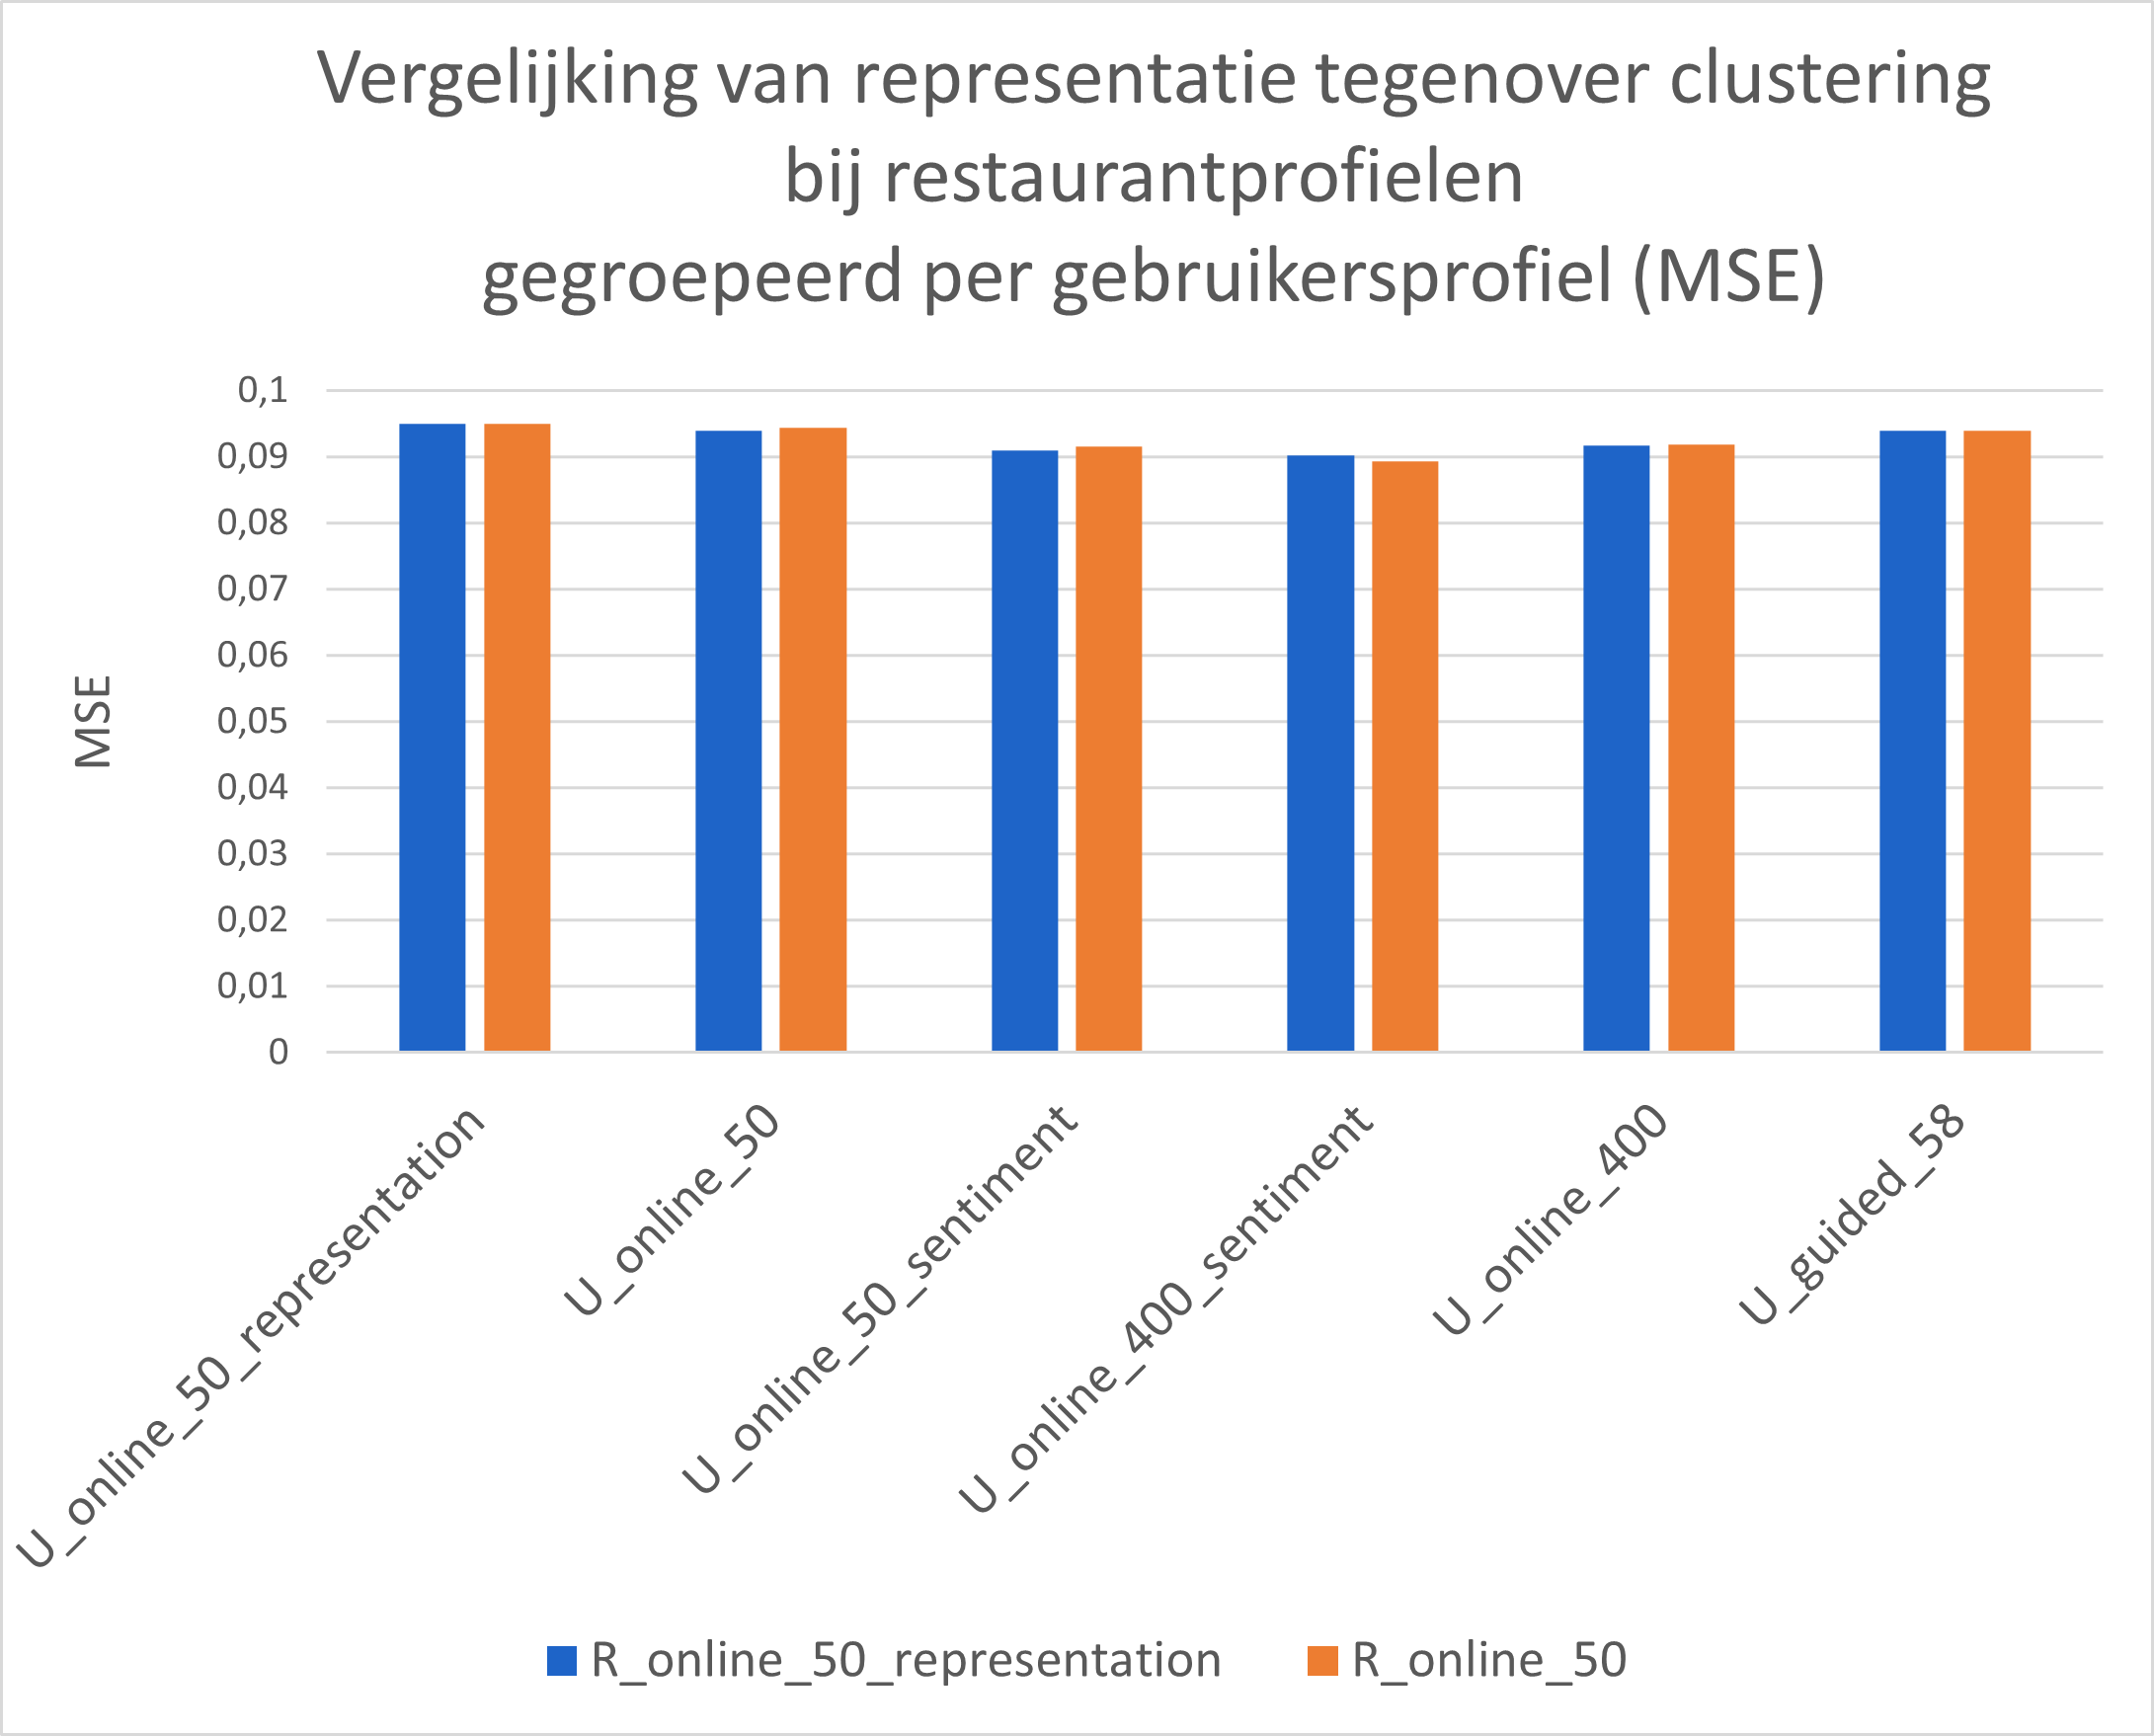
\includegraphics[width=\linewidth]{fig/chapt5/NLP/nlp_comparison_approx_restaurant.png}}\quad
        \parbox[b]{0.37\textwidth}{
        \subcaption{Restaurantprofiel op basis van representatie (blauw) en restaurantprofiel op basis van clustering (oranje) vergeleken met verschillende gebruikersprofielen op basis van MSE.}\label{fig:chapt5_nlp_approx_vs_topics_restaurant}}
        \\[.5cm]

        \caption{Analyse van de performantie van profielen op basis van clustering tegenover profielen op basis van representatie.}
        \label{fig:chapt5_nlp_approx_vs_topics}
\end{figure}

In \autoref{fig:chapt5_nlp_approx_vs_topics} vergelijken we de profielen op basis van clustering tegenover profielen op basis van representaties, zoals beschreven in \autoref{sec:chapt4_nlp_profielen}. Analoog aan sentiment analysis maken we een onderscheid tussen gebruikers- en restaurantprofielen. In \autoref{fig:chapt5_nlp_approx_vs_topics_users} vergelijken we een gebruikersprofiel op basis van clustering tegenover gebruikersprofiel op basis van representatie in combinatie met verschillende restaurantprofielen. We kunnen concluderen dat de resultaten heel gelijkaardig zijn aan elkaar. Analoog kunnen we dit doen voor restaurantprofielen, zoals weergegeven in \autoref{fig:chapt5_nlp_approx_vs_topics_restaurant}. Net zoals de gebruikersprofielen nemen we geen significante verschillen waar. 

% TODO IS "voorgedefinieerde" een correct woord? @Arno
Vervolgens vergelijken we een online model van 50 topics met een guided variant van 48 voorgedefinieerde topics en 10 extra topics. Het doel van extra topics is om de overige niet relevant informatie op te vangen. In \autoref{fig:chapt5_nlp_guided} vergelijken we beide als gebruikersprofiel in combinatie met andere restaurantprofielen en visa versa. \\

% guided vs online  \label{fig:chapt5_nlp_guided}
% A: vergelijk (kolom 2 VS 3) \label{fig:chapt5_nlp_guided_user}   
% B: vergelijk (rij 2 VS 3) \label{fig:chapt5_nlp_guided_restaurant}
\begin{figure}[H]

        \centering
        \parbox[b]{0.6\textwidth}{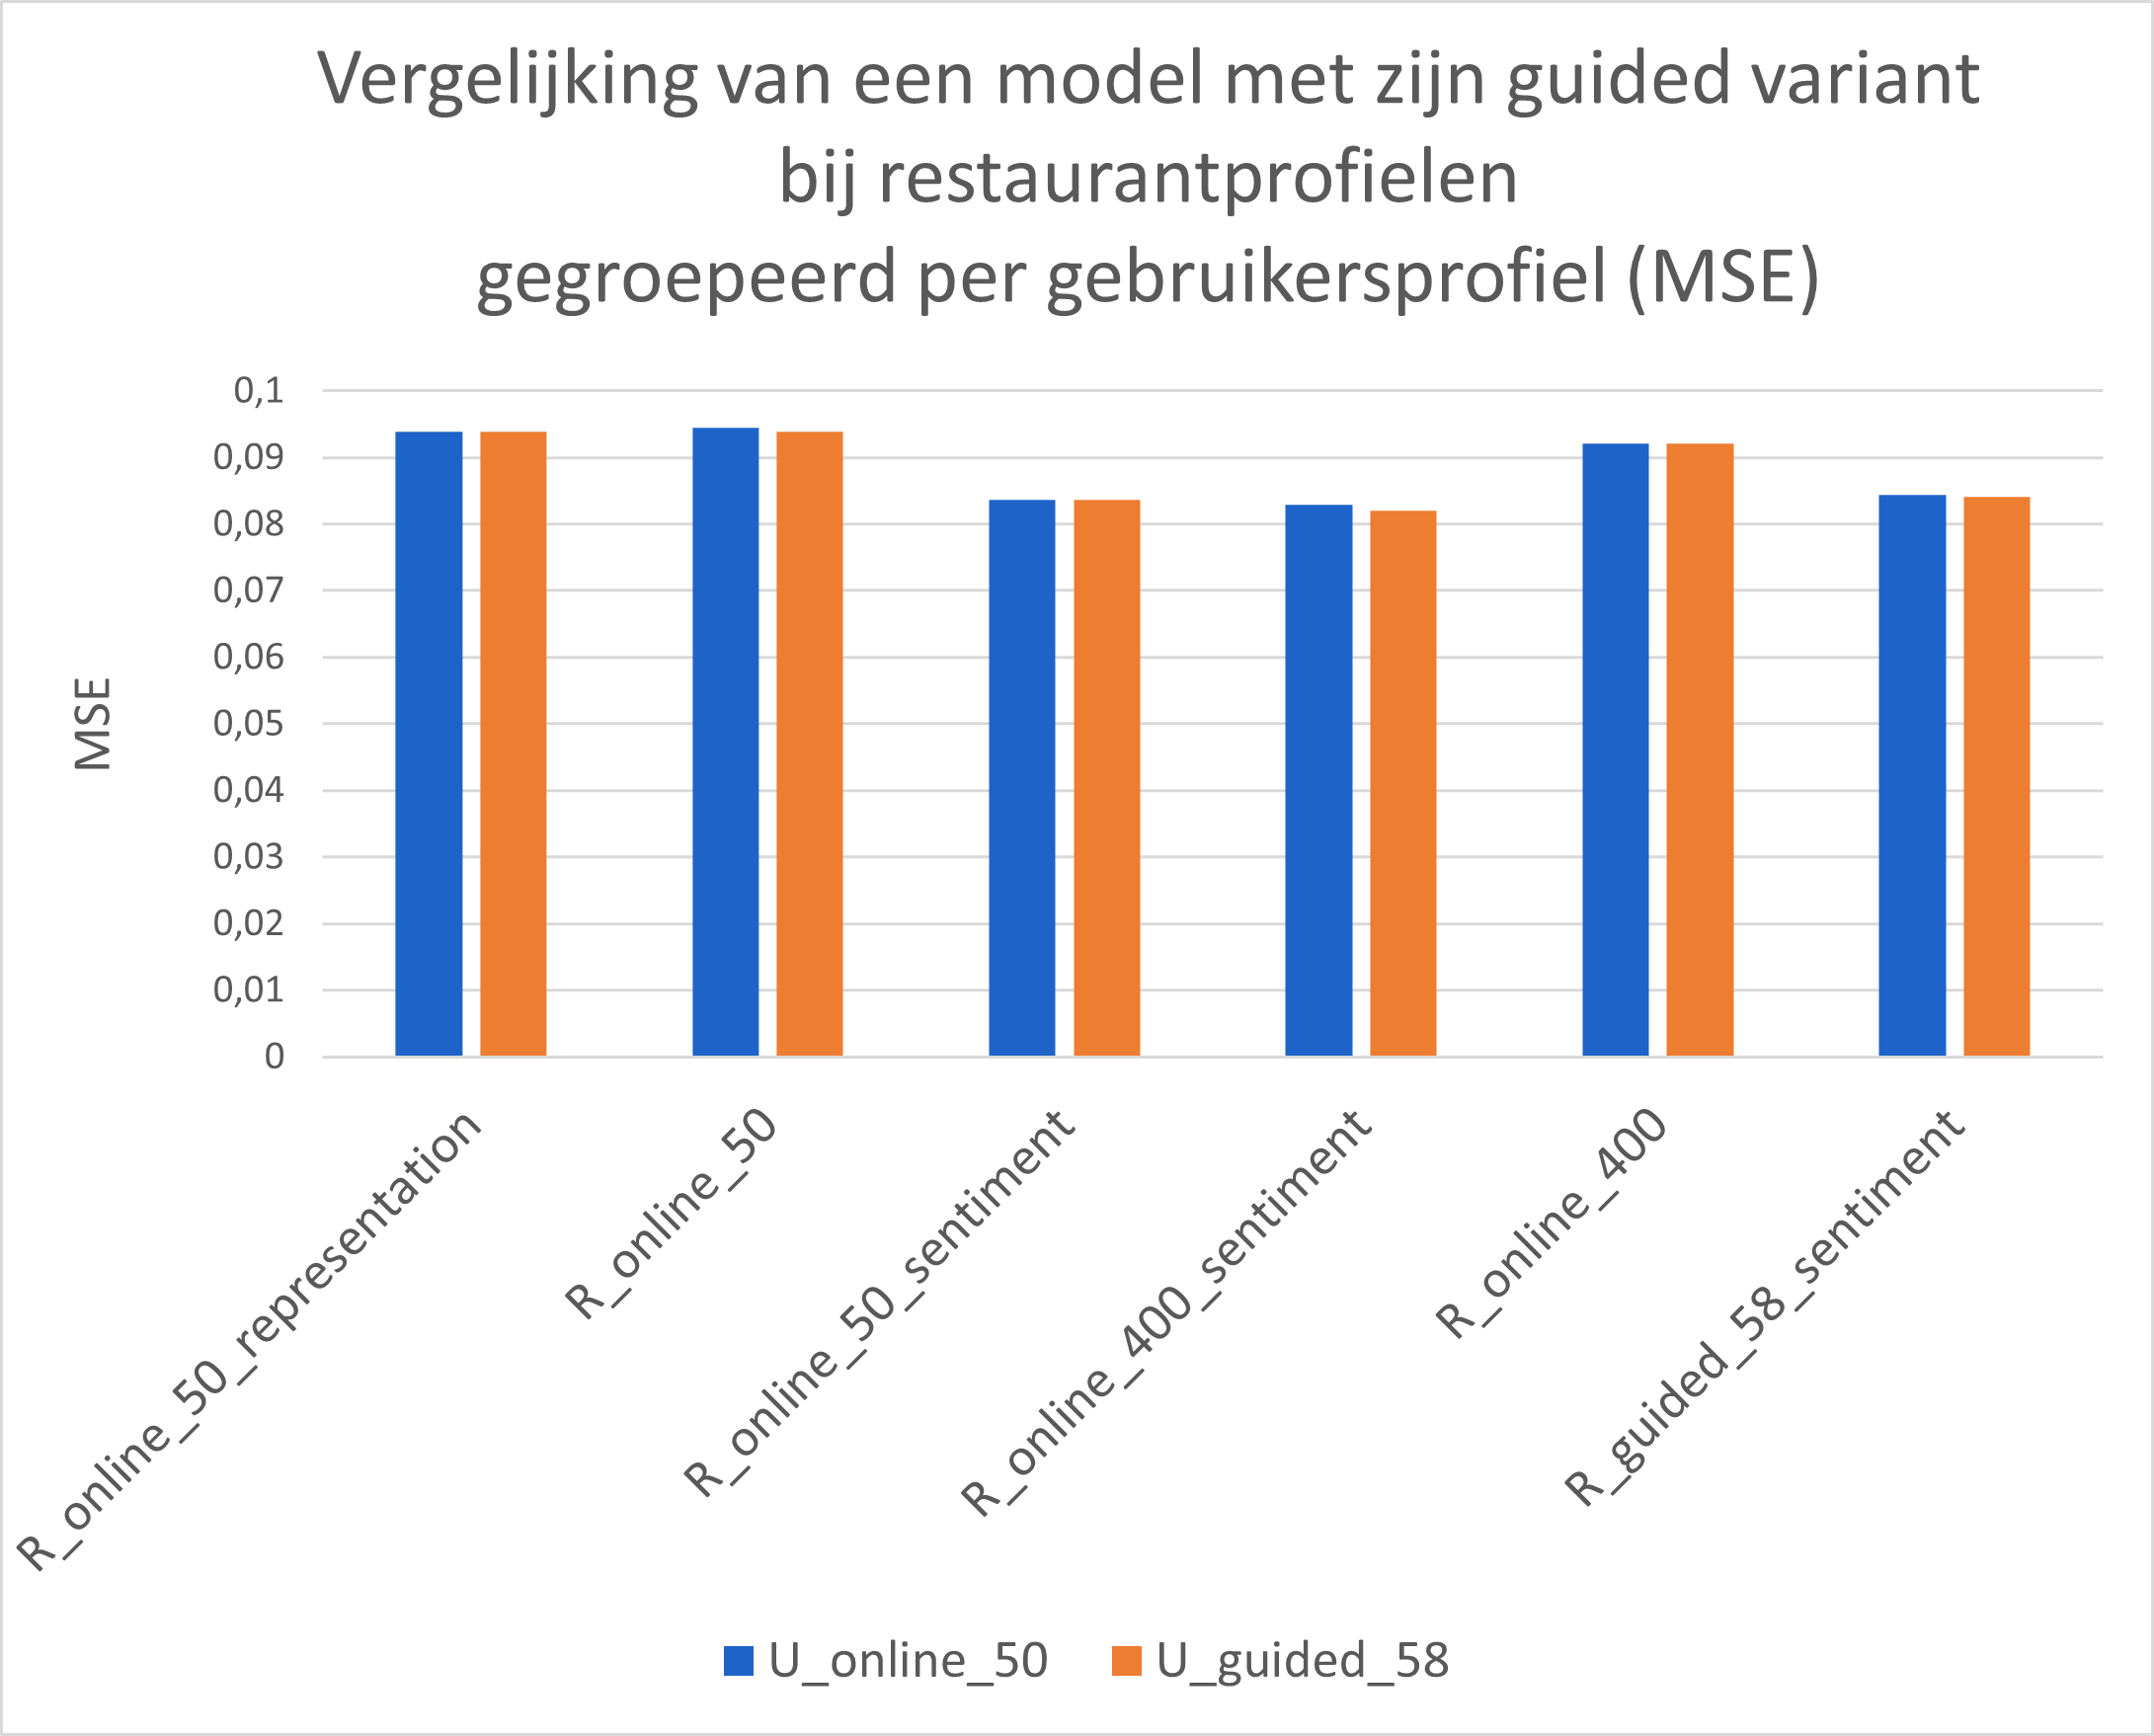
\includegraphics[width=\linewidth]{fig/chapt5/NLP/nlp_comparison_guided_gebruiker.png}}\quad
        \parbox[b]{0.37\textwidth}{
        \subcaption{Gebruikersprofiel van 50 topics (blauw) en gebruikersprofiel op basis van een guided model (oranje) vergeleken met verschillende restaurantprofielen op basis van MSE.}\label{fig:chapt5_nlp_guided_user}}
        \\[.5cm]

        \centering
        \parbox[b]{0.6\textwidth}{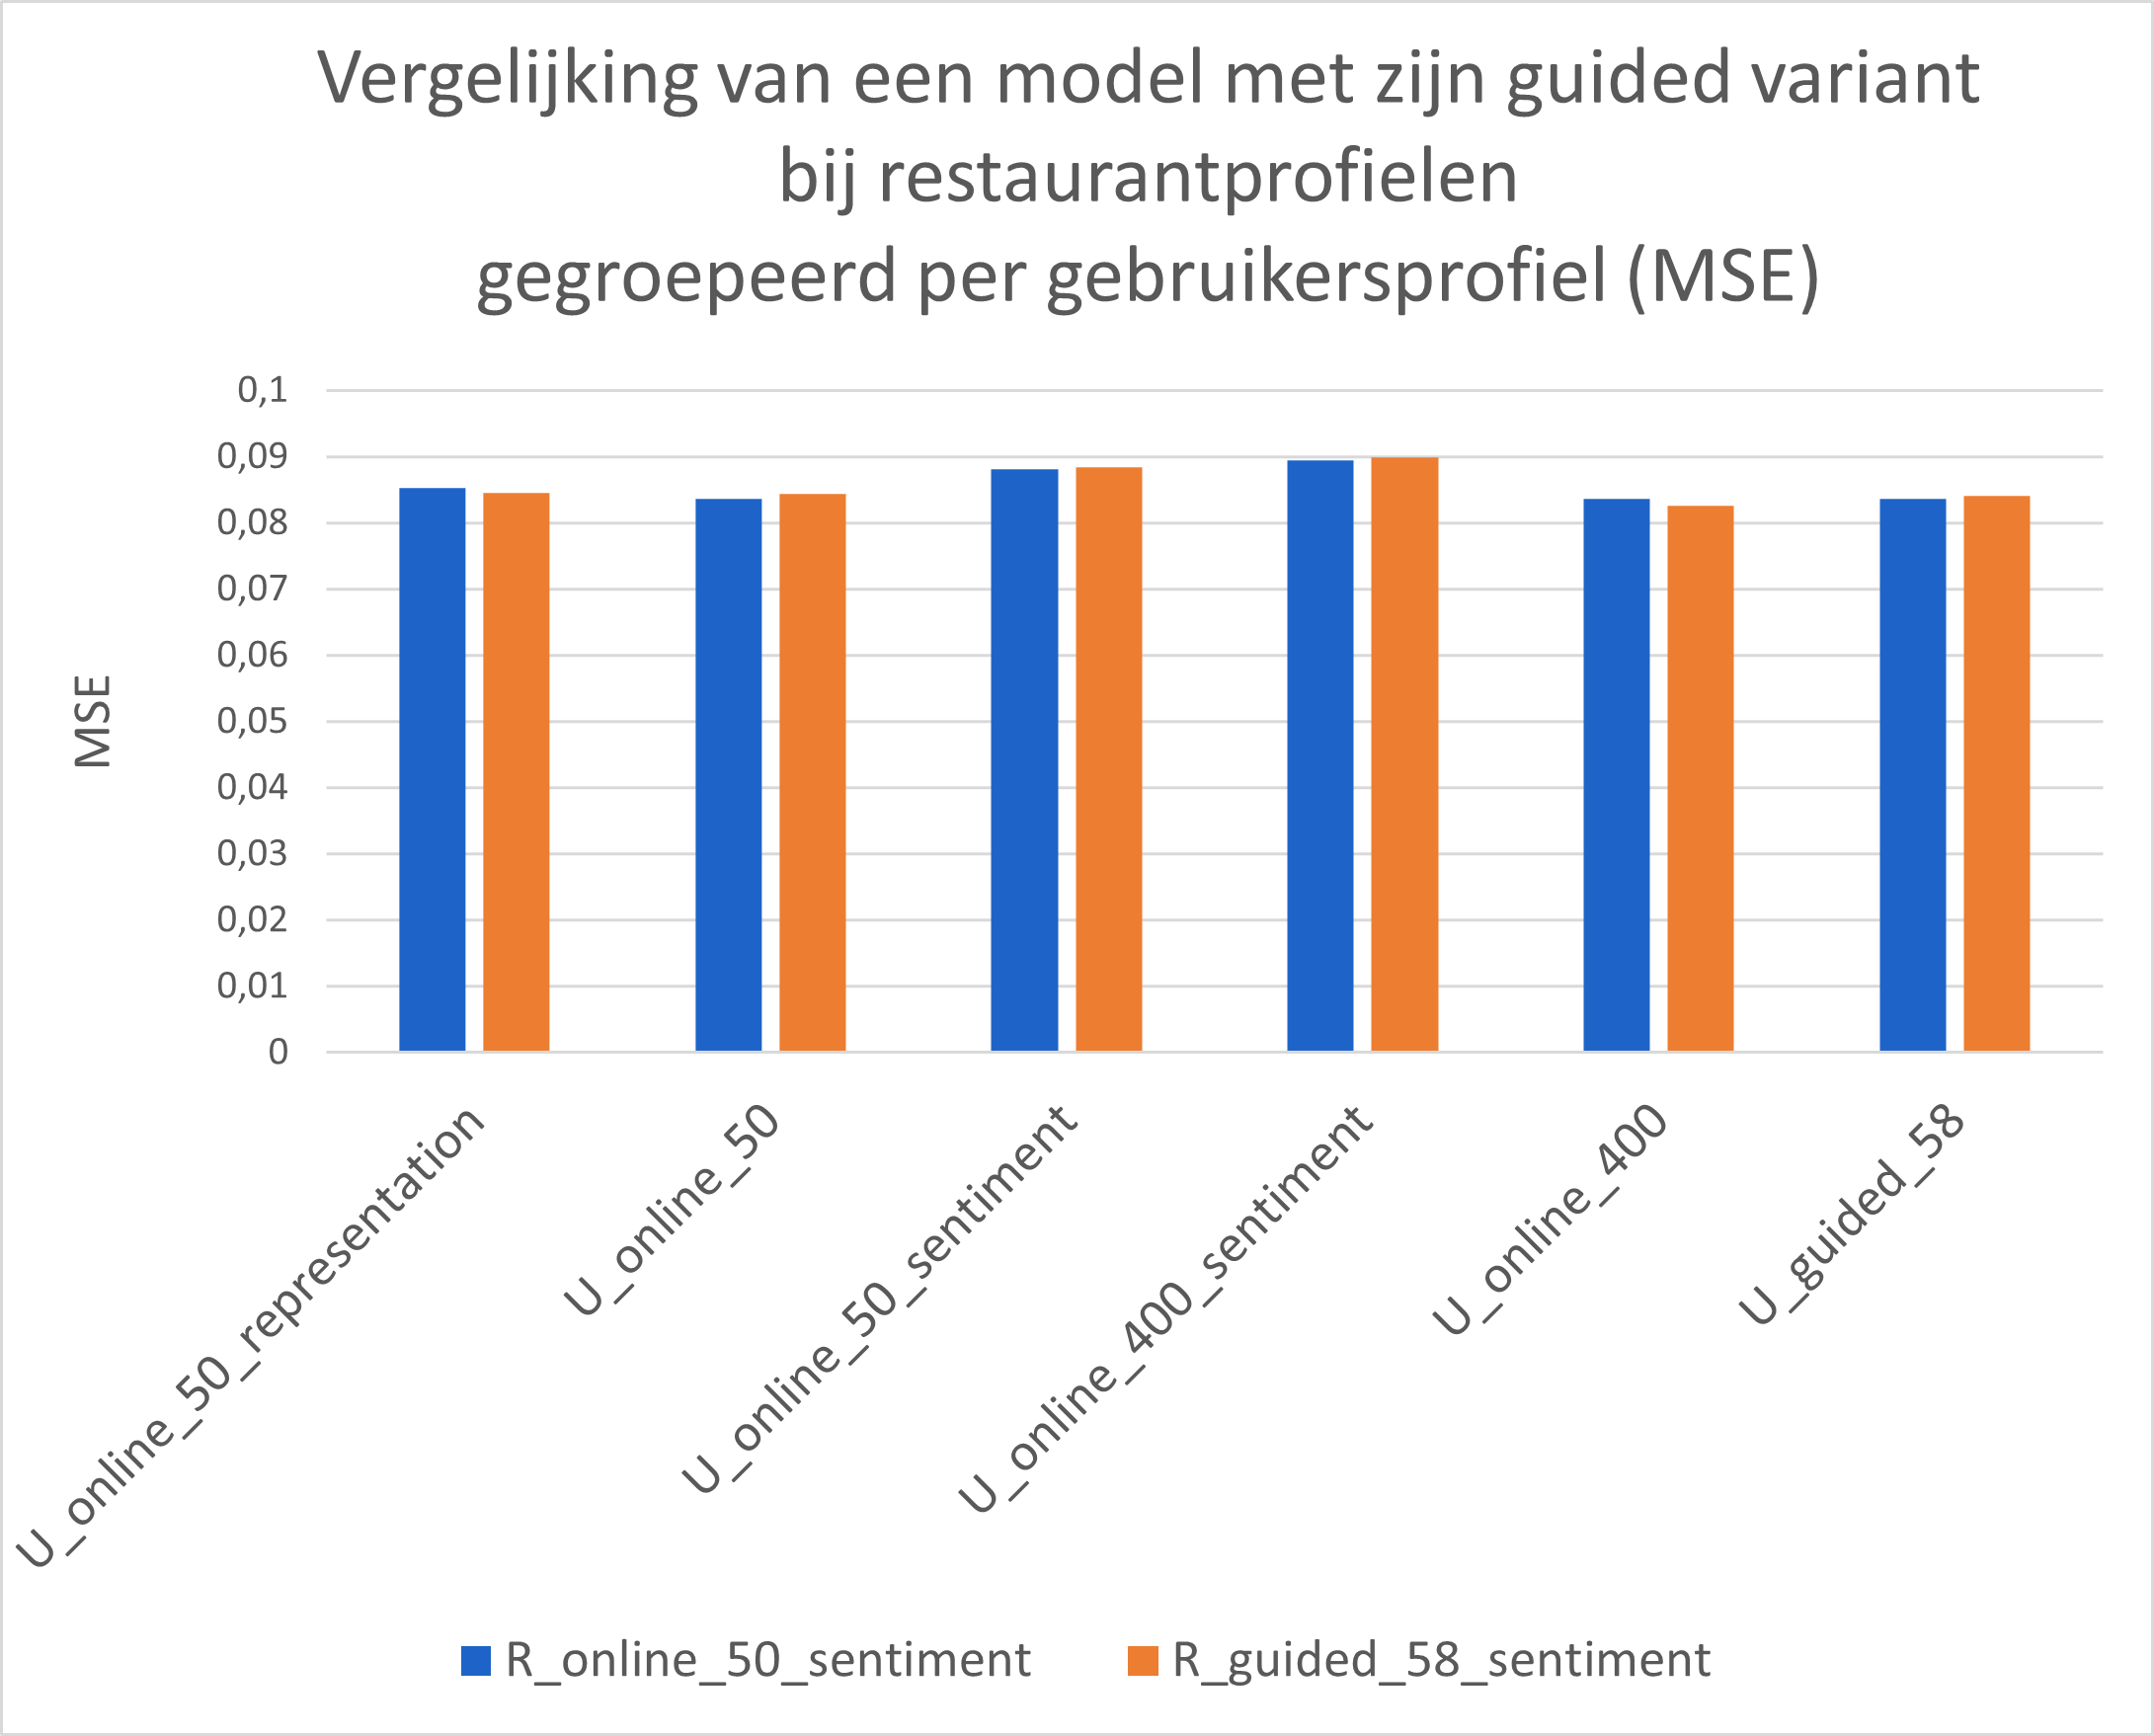
\includegraphics[width=\linewidth]{fig/chapt5/NLP/nlp_comparison_guided_restaurant.png}}\quad
        \parbox[b]{0.37\textwidth}{
        \subcaption{Restaurantprofiel van 50 topics (blauw) en restaurantprofiel op basis van een guided model (oranje) vergeleken met verschillende gebruikersprofielen op basis van MSE.}\label{fig:chapt5_nlp_guided_restaurant}}
        \\[.5cm]

        \caption{Analyse van de toegevoegde waarde van voorafgedefinieerde topics bij het genereren van gebruikers- en restaurantprofielen.}
        \label{fig:chapt5_nlp_guided}
\end{figure}

Zoals af te lezen op de grafieken in \autoref{fig:chapt5_nlp_guided} is er geen significant verschil tussen een online model en zijn guided variant. Indien we manueel naar de topics kijken vinden we weinig terug van de originele voorgedefinieerde topics. Een mogelijke verklaring is dat de hoeveelheid trainingsdata overheerst en deze topics zal overnemen. Een andere mogelijkheid is dat de voorgedefinieerde topics niet specifiek genoeg zijn waardoor er onvoldoende geconvergeerd wordt. \\

% aantal topics = lengte model = impact performance?  \label{fig:chapt5_nlp_size_model} 
% A: vergelijk (kolom 2 VS 5) \label{fig:chapt5_nlp_size_user}   
% B: vergelijk (rij 3 VS 4) \label{fig:chapt5_nlp_size_restaurant}
\begin{figure}[H]

        \centering
        \parbox[b]{0.6\textwidth}{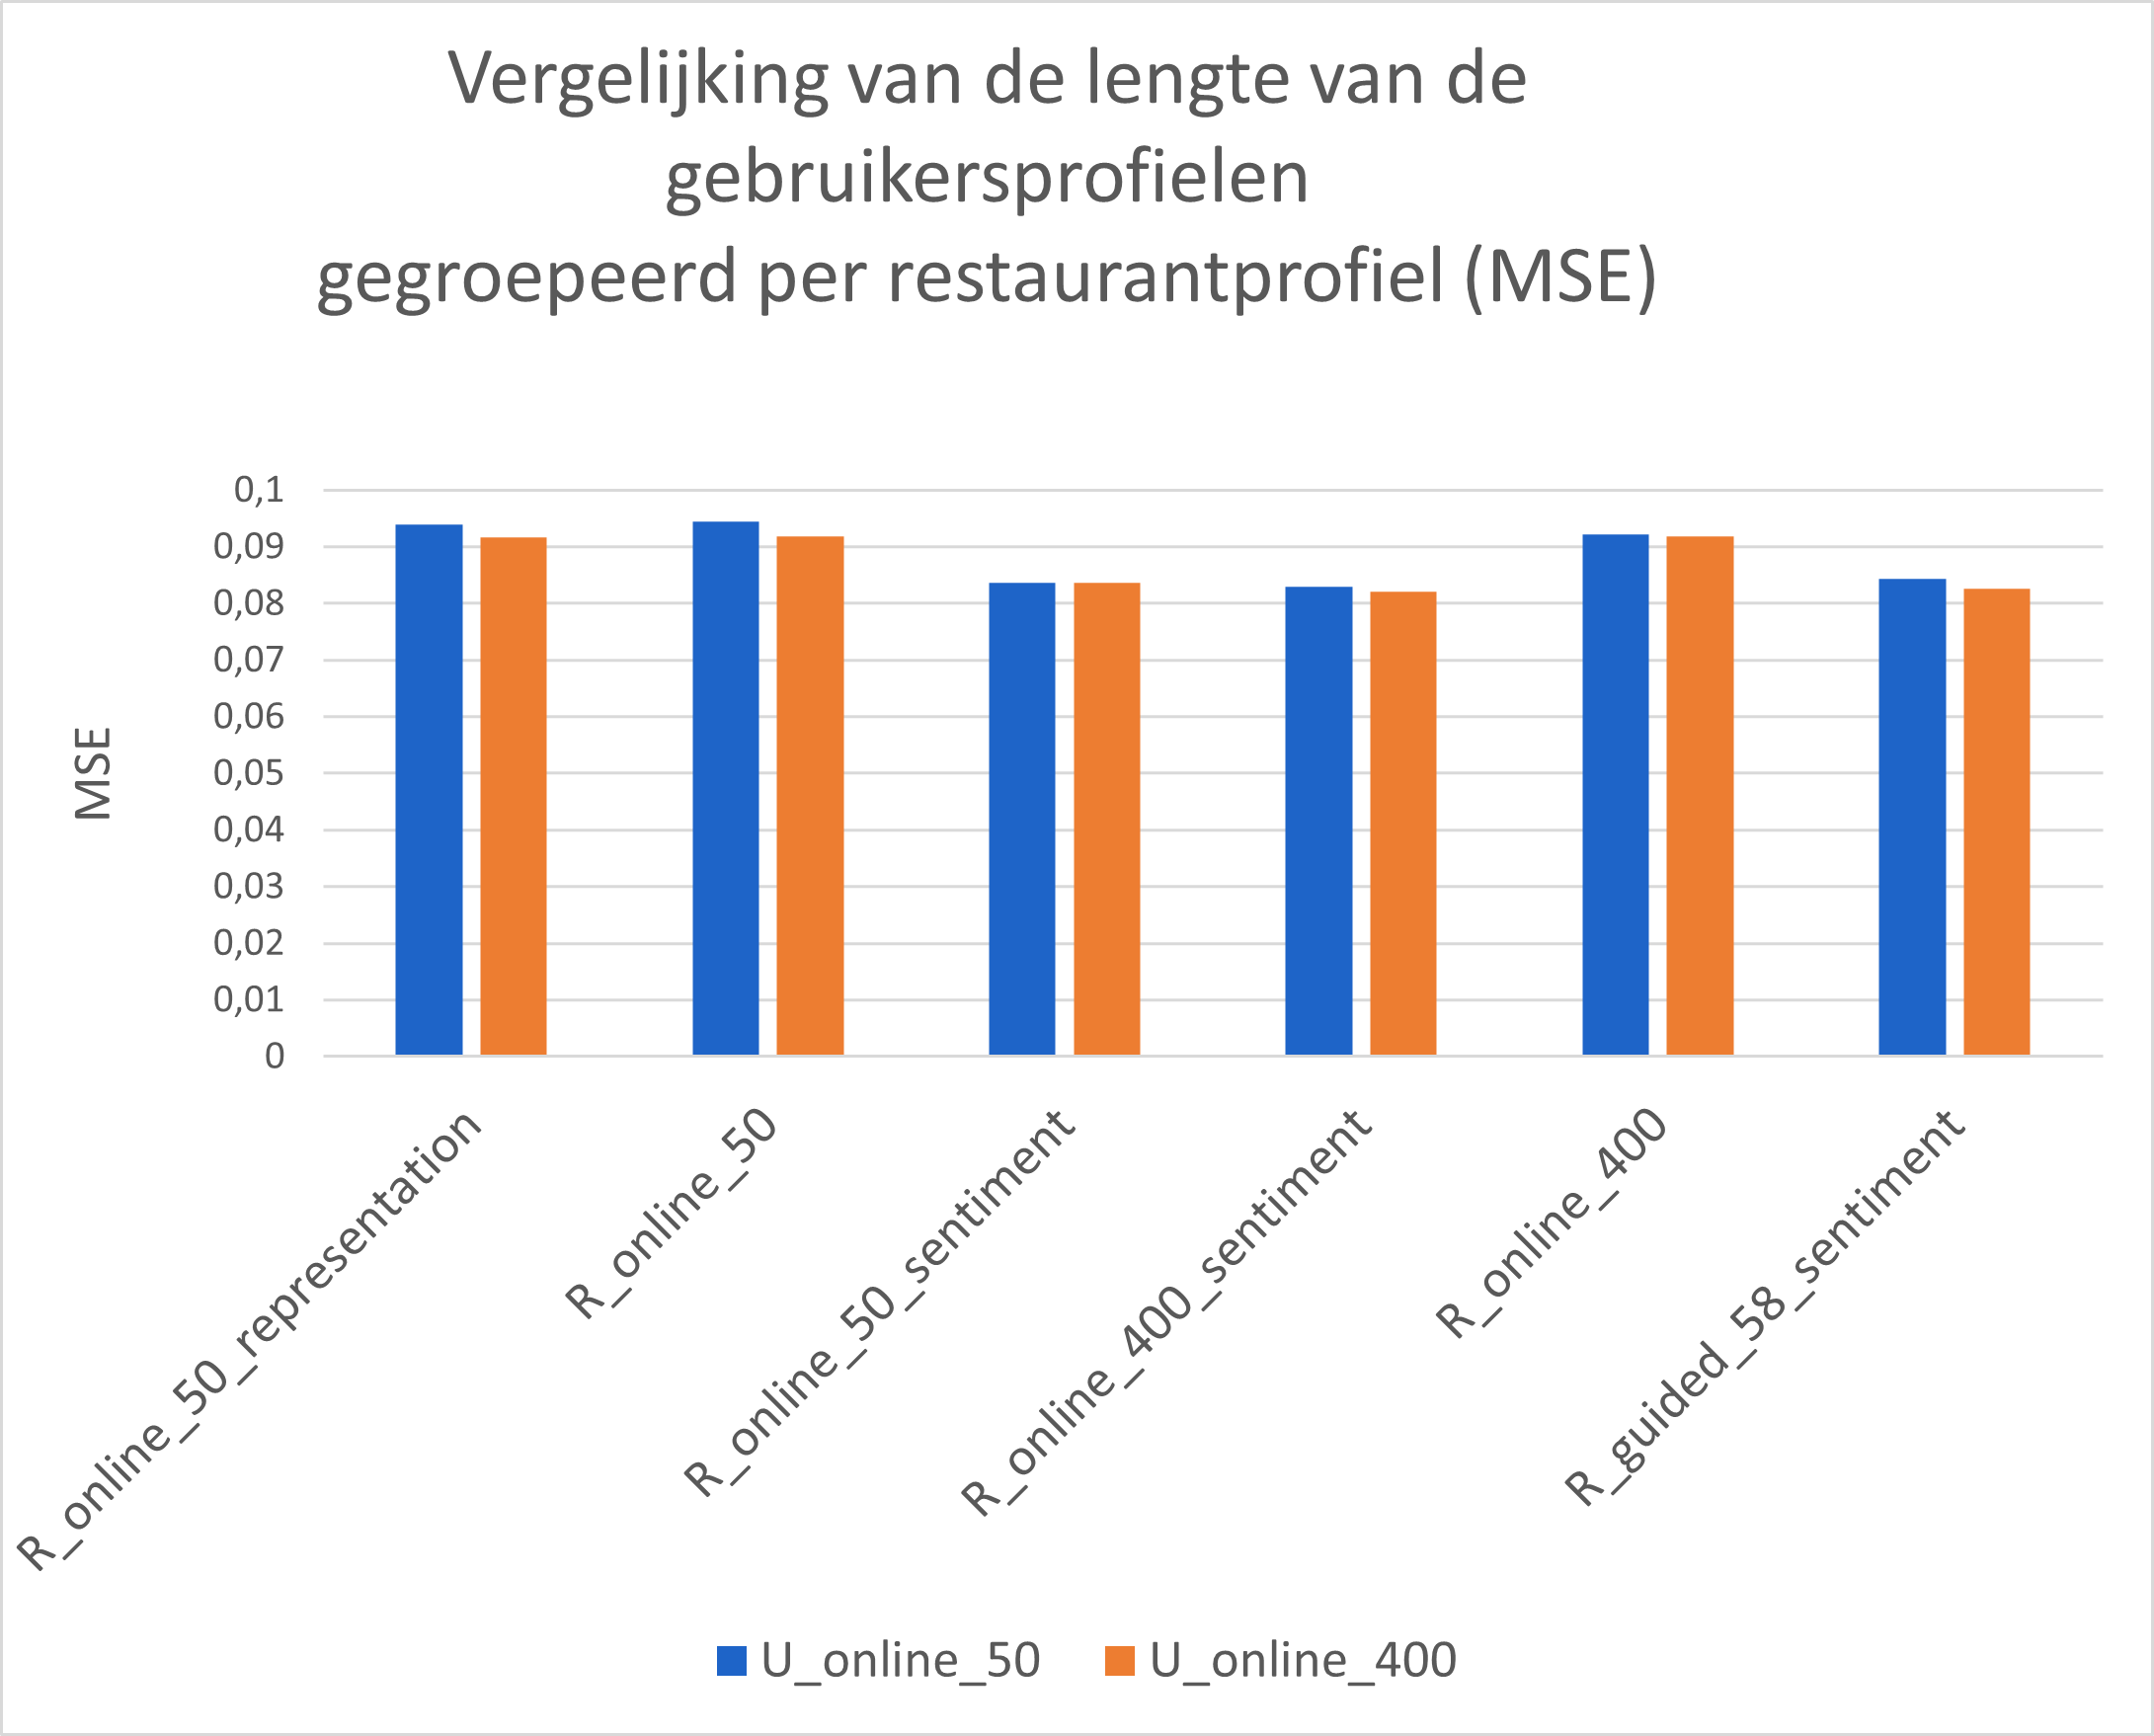
\includegraphics[width=\linewidth]{fig/chapt5/NLP/nlp_comparison_size_gebruiker.png}}\quad
        \parbox[b]{0.37\textwidth}{
        \subcaption{Gebruikersprofiel van 50 topics (blauw) en gebruikersprofiel van 400 topics (oranje) vergeleken met verschillende restaurantprofielen op basis van MSE.}\label{fig:chapt5_nlp_size_user}}
        \\[.5cm]

        \centering
        \parbox[b]{0.6\textwidth}{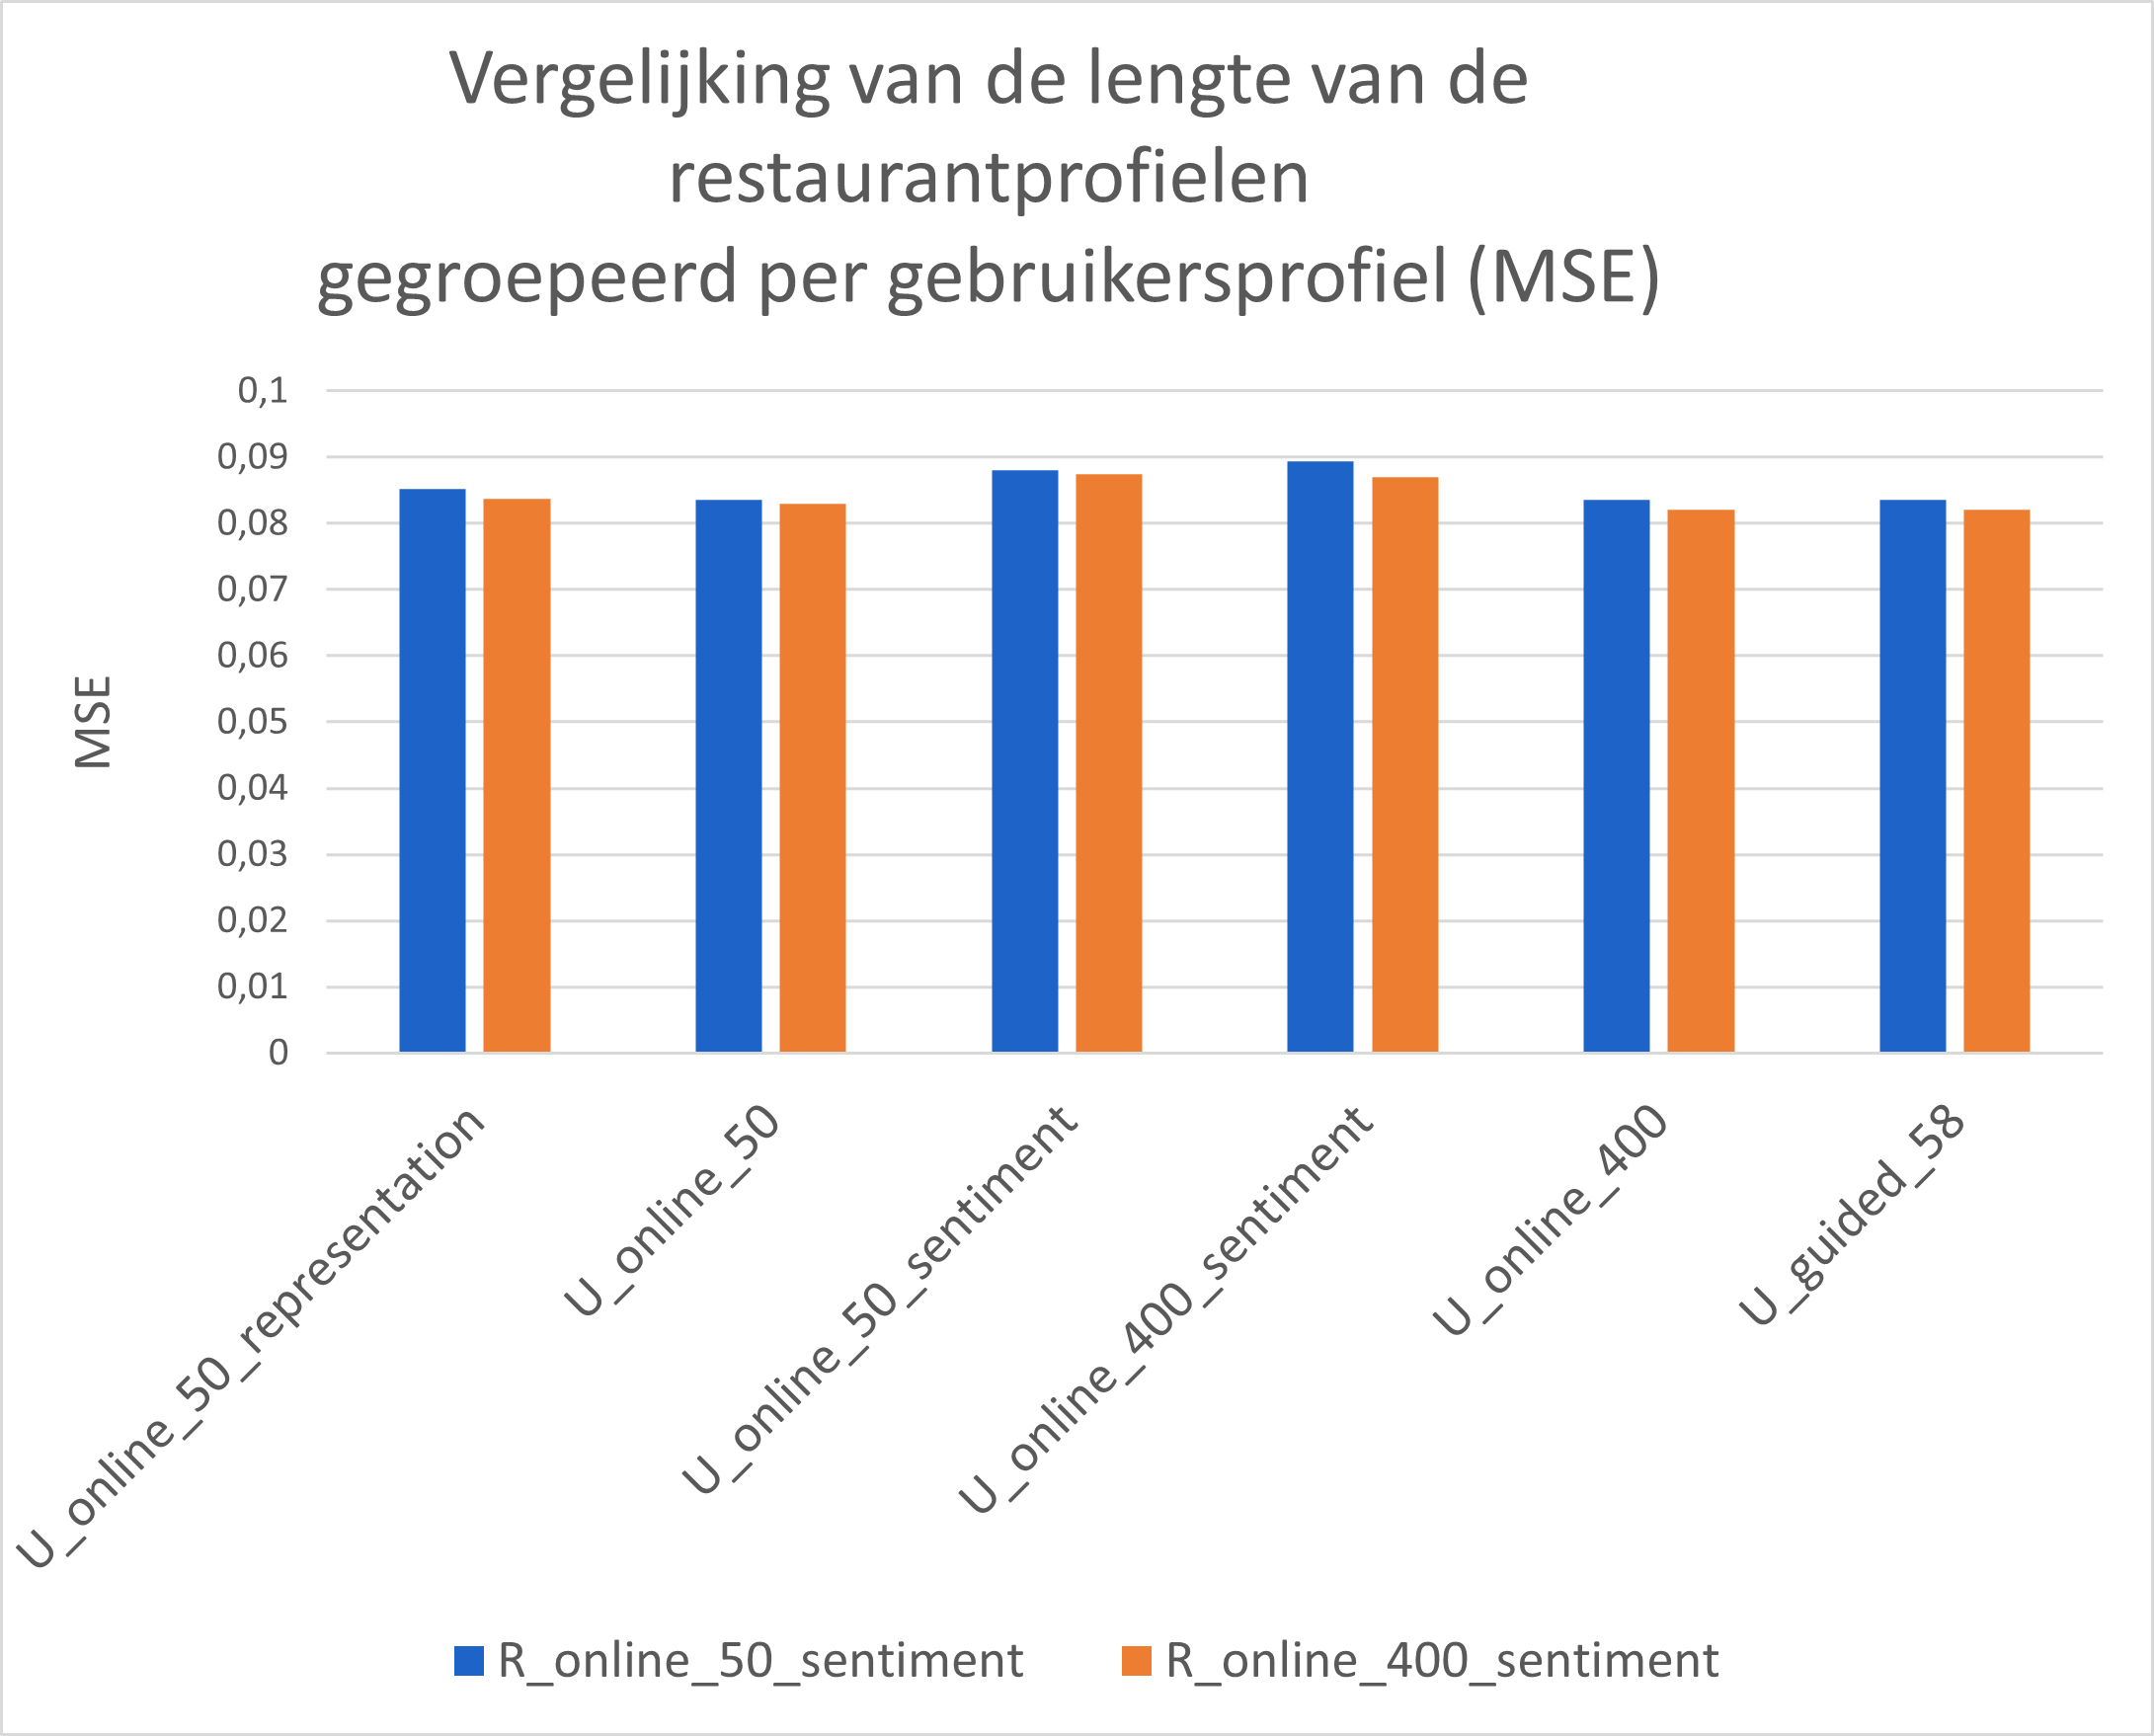
\includegraphics[width=\linewidth]{fig/chapt5/NLP/nlp_comparison_size_restaurant.png}}\quad
        \parbox[b]{0.37\textwidth}{
        \subcaption{Restaurantprofiel van 50 topics (blauw) en restaurantprofiel van 400 topics (oranje), beiden met sentiment, vergeleken met verschillende gebruikersprofielen op basis van MSE.}\label{fig:chapt5_nlp_size_restaurant}}
        \\[.5cm]

        \caption{Analyse van de impact van de lengte van gebruikers- en restaurantprofielen.}
        \label{fig:chapt5_nlp_size_model}
\end{figure}

De volgende hyperparameter die we bespreken is het aantal topics dat een model zal genereren, dit is equivalent aan de lengte van de gebruikers- en restaurantprofielen. Door het gebruik van meer topics kan het model in het ideale geval specifieker zijn per topic. Hierdoor is het mogelijk om een duidelijker beeld te krijgen van een gebruiker of restaurant. In \autoref{fig:chapt5_nlp_size_model} gaan we twee gelijke modellen, met uitzondering van het aantal topics, met elkaar vergelijken. We concluderen dat het model van 400 topics nauwelijks beter is dan het model van 50 topics. Een mogelijke verklaring is dat het embeddingsmodel van BERTopic niet gefinetuned is. Het gevolg hiervan is dat woorden zoals pasta en pizza toch in één topic samengevoegd worden. In het ideale geval worden deze afgesplitst zodat we hiervoor een onderscheid kunnen maken per gebruiker of restaurant.

Een laatste experiment is het manueel wegfilteren van bepaalde topics die niet relevant zijn voor een gebruikers- of restaurantprofiel zoals beschreven in \autoref{sub:chapt4_users_vs_restaurants}. Dit is nuttig indien we de representatie van modellen gebruiken aangezien we hier een top $n$ selecteren. In het geval dat we de clustering worden de waarden overeenkomend met de verwijderde topics op nul gezet, dit komt overeen met bepaalde features weg te laten uit een neuraal netwerk. Met deze reden zullen we dit experiment focussen op de profielen op basis van representatie. \\

% filter topics \label{fig:chapt5_nlp_filter}
\mijnfiguur[H]{width=10cm}{fig/chapt5/NLP/nlp_comparison_filter.png}{Vergelijken van profielen van 400 topics waarbij er manueel topics weggefilterd kunnen worden.}{fig:chapt5_nlp_filter}

In ons geval hebben we manueel de relevante topics geselecteerd van een online model met 400 topics. Vervolgens hebben we in \autoref{fig:chapt5_nlp_filter} de performantie van de profielen met aangepaste topics vergeleken met de originele. We maken een onderscheid tussen niet filteren, enkel gebruikersprofielen filteren, enkel restaurantprofielen filteren en ten slotte beide filteren. We merken op dat het manueel filteren van topics de performantie lichtelijk laat dalen.

We kunnen concluderen dat er meerdere mogelijkheden zijn om goede gebruikers- en restaurantprofielen te genereren. Het BERTopic model dat de beste resultaten geeft is online\_400, maar online\_50 en guided\_58 sluiten daar dichtbij aan. Ook voor de manier waarop we het model gebruiken, namelijk via de clustering of de representatie, is er weinig verschil. Het manueel wegfilteren van topics geeft extra werk met een negatieve impact op performantie, dit kunnen we dus uitsluiten voor het maken van de beste profielen. Ten slotte de meest impactvolle toevoeging is het gebruik van sentiment in de restaurantprofielen. Hiermee zien we een significante toename in performantie. \newline
Voor de experimenten in \autoref{sec:chapt5_neuraal_netwerk} maken we gebruik van de beste gebruikers- en restaurantprofielen. Beiden worden gegenereerd aan de hand van de clustering van een online\_400 model, waarbij sentiment wordt toegevoegd aan de restaurantprofielen. % TODO 400 want meer parameters voor neuraal netwerk om te experimenteren voor complexe verbanden -> is dit waar?

\subsection{Verband tussen verschillende evaluatiemethoden}
\label{sub:chapt5_compare_eval_methods}
Nu we hebben vastgelegd welke modellen goede en slechte gebruikers- en restaurantprofielen genereren kunnen we deze vergelijken met de resultaten van de clusteringsmetrieken. Ondanks het feit dat Calinski-Harabasz score efficiënt te berekenen is, hangt deze af het aantal topics waardoor het vergelijken lastig wordt. Hierdoor zullen we enkel gebruik maken van de Davies-Bouldin score en silhouette score. We gaan hier de resultaten uit \autoref{sub:chapt4_eval_clustering} vergelijken met de MSE van gebruikers- en restaurantprofielen gegenereerd aan de hand van de clustering van verschillende modellen, gecombineerd met sentiment analysis voor de restaurantprofielen. 

\mijnfiguur[H]{width=14cm}{fig/chapt5/NLP/nlp_comparison_davies.png}{Verband tussen MSE en de Davies-Bouldin score voor verschillende BERTopic modellen.}{fig:chapt5_nlp_davies}

In \autoref{fig:chapt5_nlp_davies} merken we op dat de Davies-Bouldin score en MSE in het algemeen dezelfde trend volgen. De enige uitzondering is het model online\_400\_HD, hierbij is de dimensie hoger voor het clusteren, maar dit is niet het geval de MSE die in lijn ligt met de andere goede modellen. We nemen waar dat clusteren met een hogere dimensie een aanzienlijke impact heeft op de uitkomst van de Davies-Bouldin score. 

\mijnfiguur[H]{width=14cm}{fig/chapt5/NLP/nlp_comparison_silhouette.png}{Verband tussen MSE en de silhouette score voor verschillende BERTopic modellen.}{fig:chapt5_nlp_silhouette}

De tweede metriek die we vergelijken is de silhouette score. In dit geval moeten we opletten aangezien betere MSE scores overeenkomen met lagere waarden, maar voor de silhouette score is een hogere score beter. Indien we hiermee rekening houden zien we in \autoref{fig:chapt5_nlp_silhouette} dezelfde resultaten als bij de vergelijking met de Davies-Bouldin score.

% We concluderen dat de resultaten van de clusteringsmetrieken een goede indicatie geven over de uiteindelijke performantie van een model. Hierbij moeten we opletten van factoren die deze metrieken kunnen beïnvloeden, bijvoorbeeld de grootte van de dimensie voor het clusteren. Tot slot vermelden we dat aan de hand van deze metrieken enkel de performantie van de verschillende BERTopic modellen geëvalueerd kan worden. Externe manipulaties zoals sentiment analysis kunnen niet geëvalueerd worden door deze metrieken. Hiervoor moeten we gebruik maken de evaluatiemethoden van het neuraal netwerk zoals beschreven in \autoref{sub:chapt4_testsetup}.

























% TODO: ook niet vergeten om te evalueren zonder profielen en zonder restaurantprofielen
\section{Neuraal netwerk}
\label{sec:chapt5_neuraal_netwerk}
Op dit punt hebben we aan de hand van een basisimplementatie van het neuraal netwerk de beste combinatie gevonden voor de inputprofielen. We keren eerst even terug naar de aanpassingen die we maakten aan het basismodel, zoals uitgelegd in de inleiding van dit hoofdstuk. Na het opstellen van alle mogelijke implementaties van gebruikers- en restaurantprofielen merkten we op dat het neuraal netwerk niet in staat was om verbanden te capteren. Doordat het model na meer dan 400 epochs nog heel vaak terugviel op een voorspelling van 4 op 5, leek het aangewezen om de optimizer en diens parameters aan te passen.

We probeerden verschillende learning rates met SGD, en hoewel dit een effect had op het trainingsproces, slaagden we er niet in om een geschikte waarde te vinden. Een kleine learning rate zorgde dat het model niets leerde. Bij grotere learning rates was het model zeer instabiel waardoor het geen verbeterde voorspellingscapaciteit opleverde na trainen over meerdere epochs (\autoref{fig:chapt5_sgd_slecht_loss}).

Doordat de ADAGRAD-optimizer dynamisch de learning rate kan aanpassen, is deze methode stabieler. We zien dit gedrag terug in \autoref{fig:chapt5_adagrad_goed}, waarbij we vinden dat een initiële learning rate van $0.0002$ de beste resultaten geeft. Hoewel de loss natuurlijk voor iedere combinatie van NLP-profielen anders is, blijft de conclusie wel hetzelde: SGD is te willekeurig en onstabiel, ADAGRAD is stabieler en scoort een (iets) lagere loss. Hierdoor kozen we om deze optimizer te gebruiken bij het evalueren van de NLP-profielen.

\begin{figure}[H]
    \begin{subfigure}{.45\textwidth}
        \centering
        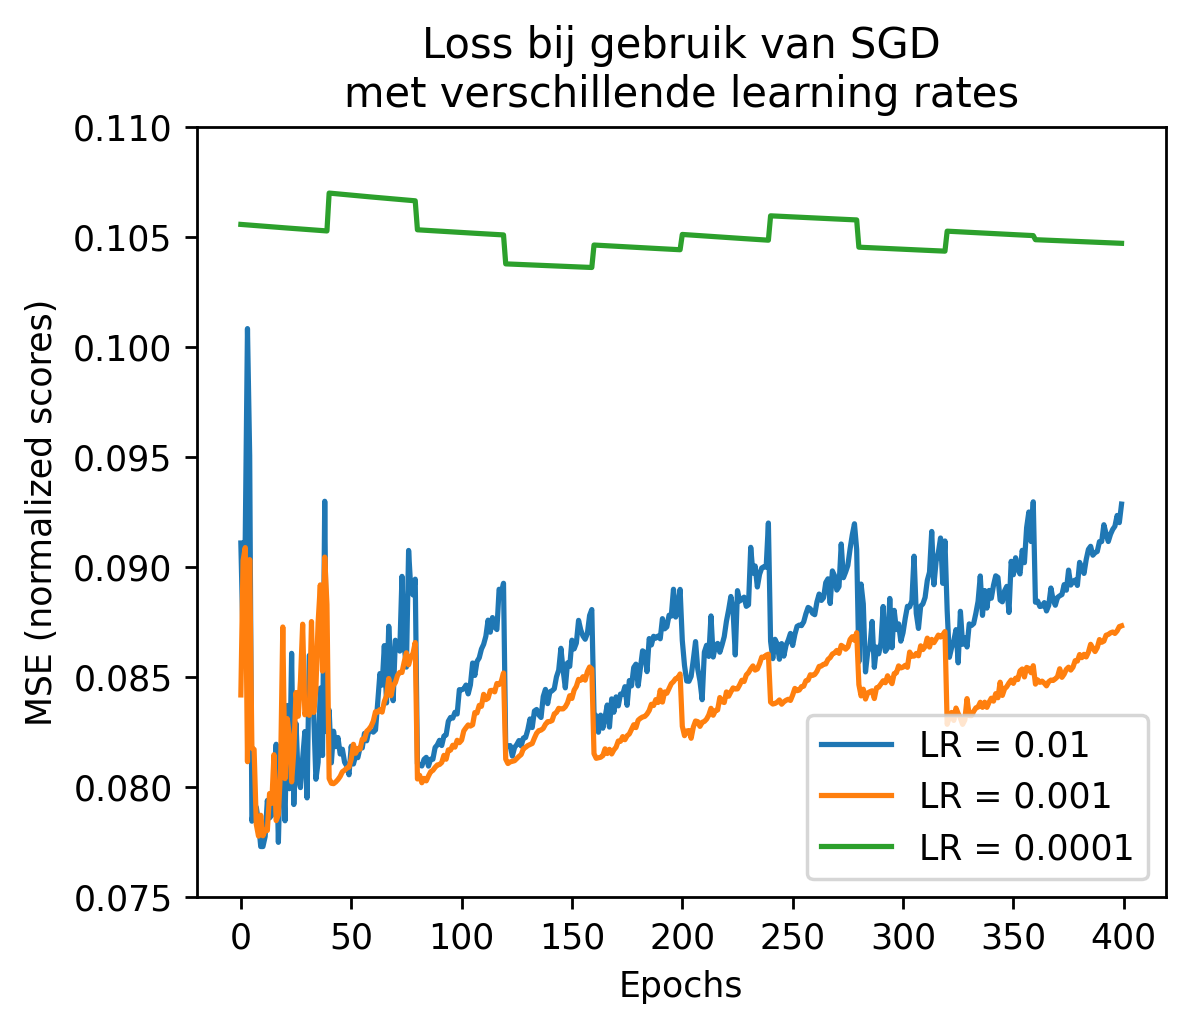
\includegraphics[width=1\linewidth]{fig/chapt5/predictor/sgd_slecht.png}
        \caption{SDG}
        \label{fig:chapt5_sgd_slecht_loss}
    \end{subfigure}
    \begin{subfigure}{.45\textwidth}
        \centering
        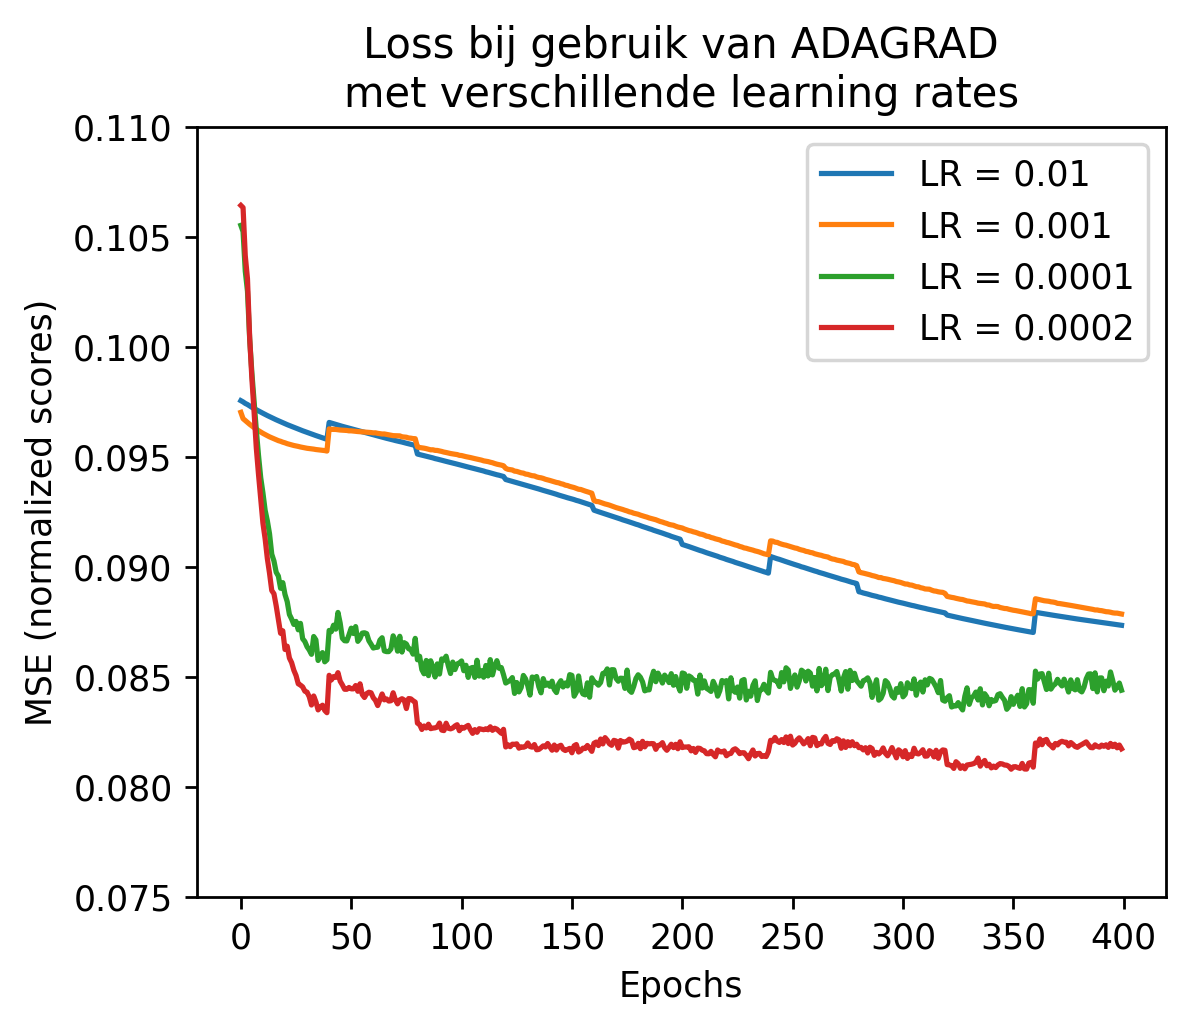
\includegraphics[width=1\linewidth]{fig/chapt5/predictor/adagrad_goed.png}
        \caption{ADAGRAD}
        \label{fig:chapt5_adagrad_goed}
    \end{subfigure}
    \caption{SGD slaagt er niet in om het model verbanden aan te leren, ADAGRAD wel}
    \label{fig:chapt5_sgd_adagrad_combined}
\end{figure}

Merk op dat naar mate het aantal afgewerkte epochs toeneemt, het hergebruiken van dezelfde datasplit minder effectief wordt bij (ADAGRAD, $0.0002$). Bij deze modellen is dezelfde datasplit steeds 40 epochs op rij gebruikt. We nemen hieruit mee dat er frequenter van datasplit mag veranderd worden.\newline
Alle volgende experimenten zullen we alleen toepassen op de netwerken getraind met de best beschikbare inputvector, die onder andere bestaat uit de gebruikers- en restaurantprofielen zoals beschreven in \autoref{sub:chapt5_nlp_resultaten}.

In de volgende secties onderzoeken we verschillende eigenschappen en parameters van het neuraal netwerk. We maken hierbij de assumptie dat parameters onafhankelijk zijn van elkaar, en dat we deze individueel kunnen optimaliseren. In realiteit zal dit niet altijd kloppen. Echter zou een volledige grid search over alle parameters en inputprofielen computationeel veel te zwaar zijn.

\subsection{Architectuur neuraal netwerk}
De complexiteit van het netwerk heeft een directe impact op de performantie. De uitgebreidere netwerken scoren betere resultaten. Het beste resultaat wordt gescoord door het model met zes verborgen lagen. Merk op dat er vanaf het model met vijf verborgen lagen een merkbare sprong zit in de resultaten. Dit komt waarschijnlijk doordat de eerste verborgen laag van deze modellen meer neuronen bevat dan de inputlaag. Dit lijkt een zeer positieve invloed te hebben op de resultaten.

\mijnfiguur[H]{width=16cm}{fig/chapt5/predictor/loss_verschillende_architecturen.png}{Vergelijking van verschillende architecturen}{fig:chapt5_loss_verschillende_architecturen}

We definiëren een voorspelling als \q{correct} als de voorspelde waarde na afronding gelijk is aan de echte waarde. Deze afronding weerspiegelt de mogelijke waarden waaruit de gebruiker kan kiezen. De accuraatheid van een model is dan het percentage van correcte voorspellingen. Een analyse van de voorspellingen toont aan dat er een verband is tussen de loss en de accuraatheid van een model. Hoewel dit intuïtief klinkt, kan het zijn dat een model consistent 1 ster naast de echte waarde voorspelt, en toch een lage loss behaalt. Dit is bij ons niet het geval. \autoref{fig:chapt5_accuracy_all_architectures} toont aan dat de complexere modellen een hogere accuraatheid scoren, in lijn met het verschil in loss (\autoref{fig:chapt5_loss_verschillende_architecturen}). \autoref{fig:chapt5_accuracy_6_layers} toont de gemaakte fouten bij het beste model. We zien dat het model hoofdzakelijk een fout van 1 ster maakt.

\begin{figure}[H]
    \begin{subfigure}{.45\textwidth}
        \centering
        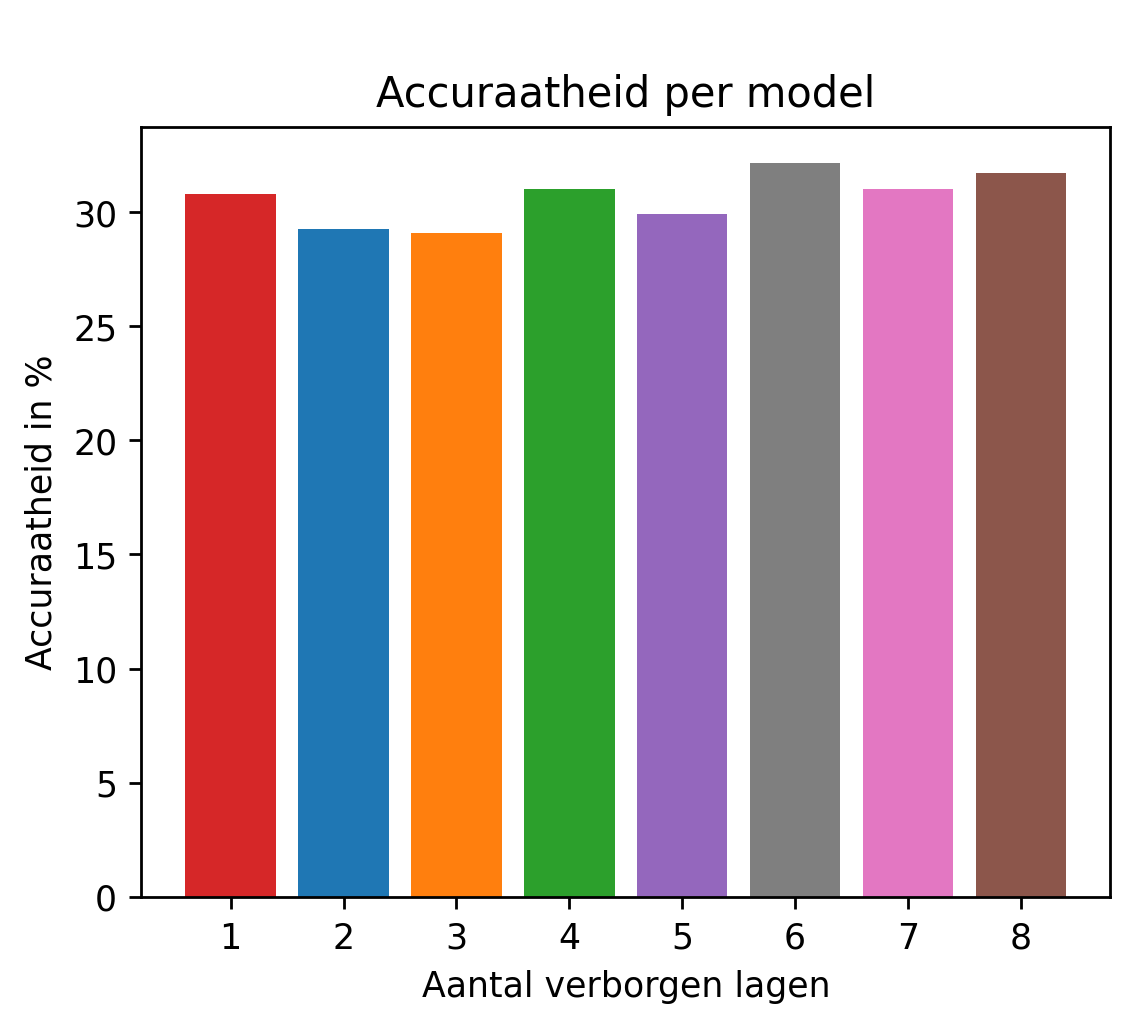
\includegraphics[width=1\linewidth]{fig/chapt5/predictor/accuracy_per_model.png}
        \caption{De accuraatheid van iedere architectuur}
        \label{fig:chapt5_accuracy_all_architectures}
    \end{subfigure}
    \begin{subfigure}{.45\textwidth}
        \centering
        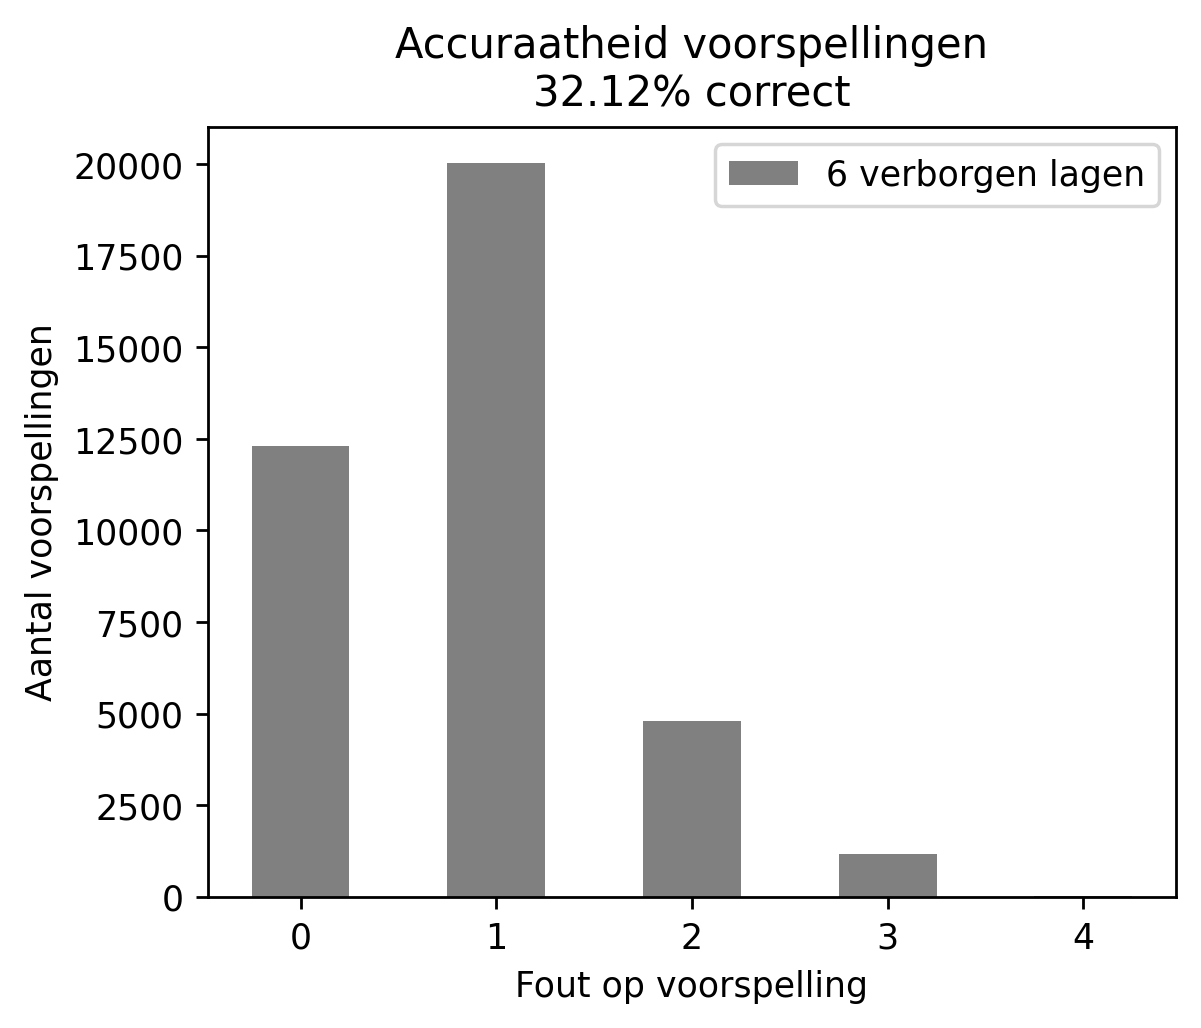
\includegraphics[width=1\linewidth]{fig/chapt5/predictor/accuracy_32.12_6_layers_hist.png}
        \caption{Histogram fouten bij model met 6 verborgen lagen}
        \label{fig:chapt5_accuracy_6_layers}
    \end{subfigure}
    \caption{Accuraatheid van modellen}
    \label{fig:chapt5_accuracy_architectures}
\end{figure}


Ieder model, inclusief het meest eenvoudige, lijkt wel effectief te leren op basis van de inputfeatures, en voorspelt dus niet steeds naïef 4 van de 5 sterren. Zo zien we de voorspellingen van het model met één verborgen laag terug in \autoref{tab:chapt5_simpel_model_voorspellingen}. Merk op dat we de voorspellingen afronden. 

\begin{table}[H]
    \centering
    \begin{tabular}{l|l|l|l}
       & Voorspelling & Echte waarde & Verschil   \\ \hline
    0  & 4            & 3            & \textbf{1} \\
    1  & 4            & 3            & \textbf{1} \\
    2  & 4            & 4            & \textbf{0} \\
    3  & 4            & 4            & \textbf{0} \\
    4  & 5            & 4            & \textbf{1} \\
    5  & 3            & 2            & \textbf{1} \\
    6  & 3            & 2            & \textbf{1} \\
    7  & 4            & 4            & \textbf{0} \\
    8  & 4            & 5            & \textbf{1} \\
    9  & 4            & 4            & \textbf{0} \\
    10 & 5            & 5            & \textbf{0}
    \end{tabular}
    \caption{Voorspellingen voor het model met 1 verborgen laag}
    \label{tab:chapt5_simpel_model_voorspellingen}
\end{table}




We stellen ook opnieuw het effect vast van het hergebruiken van dezelfde inputvectoren iedere 20 epochs: er is een klein maar meetbaar verschil in MSE. De veronderstelling dat we meerdere epochs kunnen trainen met dezelfde datasplit blijft wel gelden: we zien bijvoorbeeld dat de loss daalt tussen epoch 80 en 100 hoewel we trainen op dezelfde data, en we zien dat er toch een generaliteit wordt aangeleerd omdat bij een volgende datasplit het verschil in loss beperkt blijft.\newline
Bij de complexere modellen is er al sprake van convergentie bij de loss na ongeveer 100 epochs. Bij de modellen met maximaal vier verborgen lagen is dit pas na meer dan 250 epochs het geval. Dit ligt niet in lijn met een veronderstelde eigenschap van deze neurale netwerken, die stelt dat complexere netwerken trager convergeren tijdens het trainen. We vinden geen verklaring voor dit fenomeen.

We concluderen dat de beste resultaten worden behaalt met een model dat bestaat uit 6 verborgen lagen. De volledige architectuur ziet er dan uit als in \autoref{fig:chapt5_best_network}.

\mijnfiguur[H]{width=16cm}{fig/chapt5/predictor/best_network.png}{Voorstelling van architectuur met zes verborgen lagen, waarbij $n$ het aantal inputfeatures voorstelt}{fig:chapt5_best_network}



% TODO: controleren dat er niet te veel van de ""uitleg"" in hoofdstuk 5 staat die eigenlijk in hoofdstuk 4 moet staan


\subsection{Invloed NLP-profielen}
\label{sec:chapt5_invloed_nlp_profielen}
We bestuderen de impact van de NLP-profielen op de loss van het neuraal netwerk. Eerst meten we hoe goed het netwerk presteert zonder deze extra inputfeatures. Met andere woorden, we baseren de voorspellingen enkel op de gelabelde dataset. We proberen ook combinaties, waarbij enkel de NLP-gebruikersprofielen of NLP-restaurantprofielen worden toegevoegd aan de gelabelde data. De resultaten staan in \autoref{fig:chapt5_invloed_NLP}. We merken op dat de NLP-gebruikersprofielen een veel grotere impact hebben dan de NLP-restaurantprofielen. Het lijkt er dus op dat de gelabelde data de restaurants reeds voldoende beschrijft om verbanden te maken. Aangezien we op zoek zijn naar de best mogelijke performantie, gaan we verder met de combinatie van gebruikers- en restaurantprofielen gemaakt met zowel gelabelde als tekstuele data.

\mijnfiguur[H]{width=14cm}{fig/chapt5/predictor/invloed_NLP.png}{Loss voor verschillende combinaties van NLP-profielen}{fig:chapt5_invloed_NLP}


\subsection{Dimensionaliteitsreductie}
De huidige implementatie van het neuraal netwerk heeft een inputlaag bestaande uit $1000$ neuronen, waarvan 200 verbonden worden met gelabelde data, en 800 met NLP-profielen. We passen PCA toe op de volledige inputvector, om zo een dimensionaliteitsreductie van 1000 naar 400 uit te voeren. We onderzoeken ook PCA op enkel het NLP-restaurantprofiel, aangezien we in \autoref{sec:chapt5_invloed_nlp_profielen} ontdekten dat dit profiel relatief weinig invloed had op de voorspellingen, maar wel dimensie 400 heeft. PCA verkleint in dit geval de dimensie tot 150. Deze waarden stellen meer dan een halvering van dimensie voor, maar zijn overigens arbitrair gekozen. Uit \autoref{fig:chapt5_invloed_pca} besluiten we dat deze toepassing van PCA geen significante verbetering met zich meebrengt.

\mijnfiguur[H]{width=14cm}{fig/chapt5/predictor/invloed_pca.png}{Loss na toepassing van PCA op (een deel van) de inputvectors}{fig:chapt5_invloed_pca}


\subsection{Cold-Startprobleem}
We meten een stijging in accuraatheid bij gebruikers met meer reviews. Over de volledige dataset halen we een accuraatheid van 32,2\%. Bij gebruikers met maximaal vijf reviews ligt de accuraatheid op 22,01\%. Er is dus een significant verschil. De accuraatheid stijgt als het aantal reviews ook toeneemt. We merken op dat er percentueel minder grote voorspellingsfouten voorkomen bij gebruikers met veel reviews. Een grotere hoeveelheid data per gebruiker biedt dus meer zekerheid. In een productieomgeving zouden we voor gebruikers met minder dan vijf reviews een aanpassing aan het model voorstellen: hierbij zouden populaire restaurants met een hoge gemiddelde score een groter gewicht hebben bij het genereren van aanbevelingen, daar ons model nog niet veel zekerheid kan bieden voor deze gebruikers.

Het is ook mogelijk dat gebruikers met veel reviews meer belang hechten aan hun Yelpaccount, en daarom meer kwalitatieve reviews achterlaten waar de NLP-algoritmen meer data uit kunnen extraheren.


\mijnfiguur[H]{width=10cm}{fig/chapt5/predictor/effect_coldstart_partities.png}{Evolutie in accuraatheid bij stijgend aantal reviews per gebruiker}{fig:chapt5_coldstart_partities}

\begin{figure}[H]
    \begin{subfigure}{.45\textwidth}
        \centering
        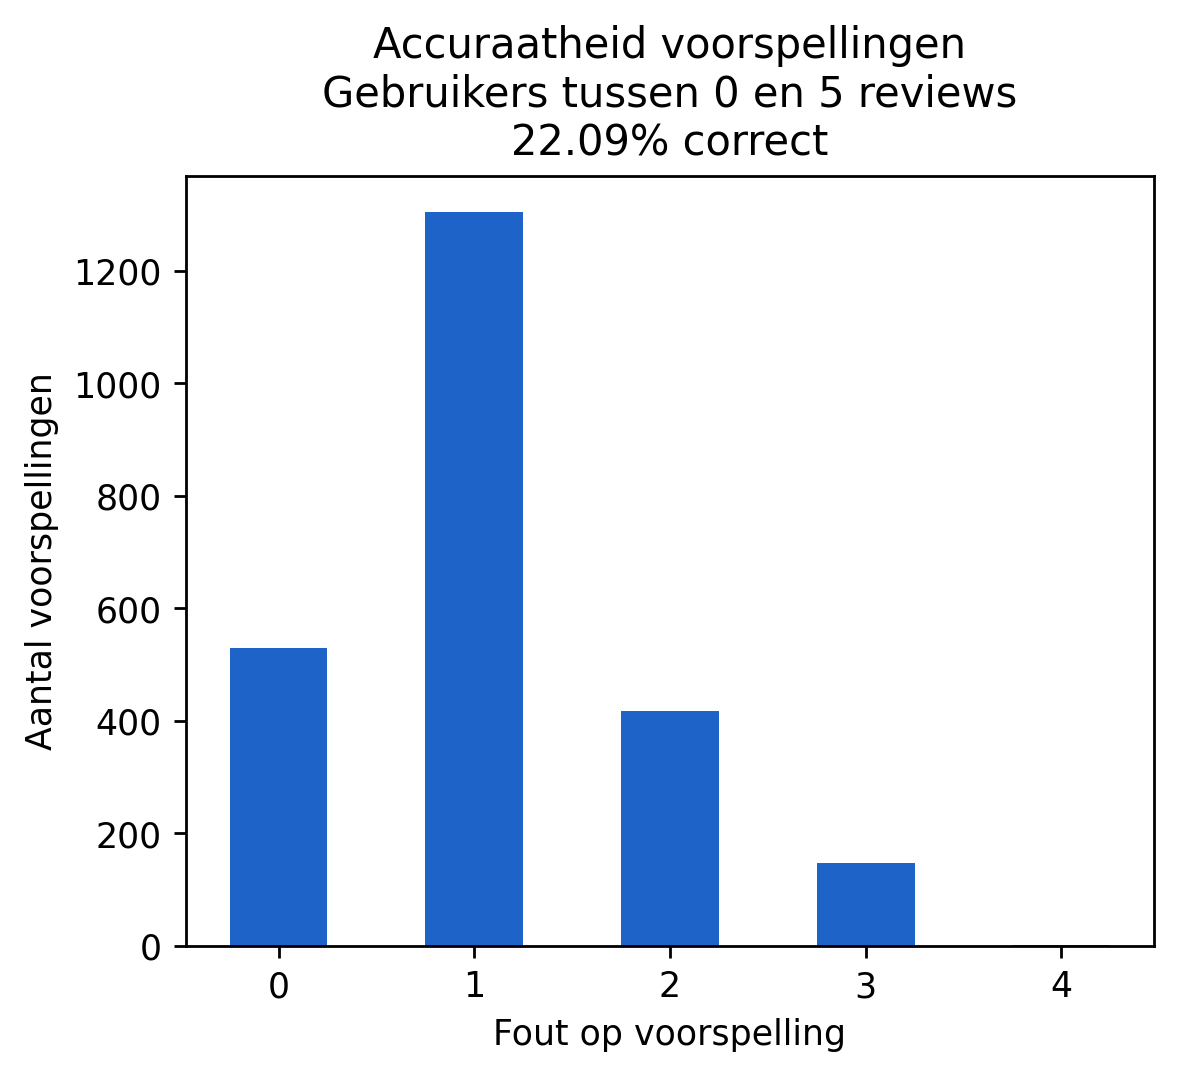
\includegraphics[width=1\linewidth]{fig/chapt5/predictor/accuracy_0_5.png}
    \end{subfigure}
    \begin{subfigure}{.45\textwidth}
        \centering
        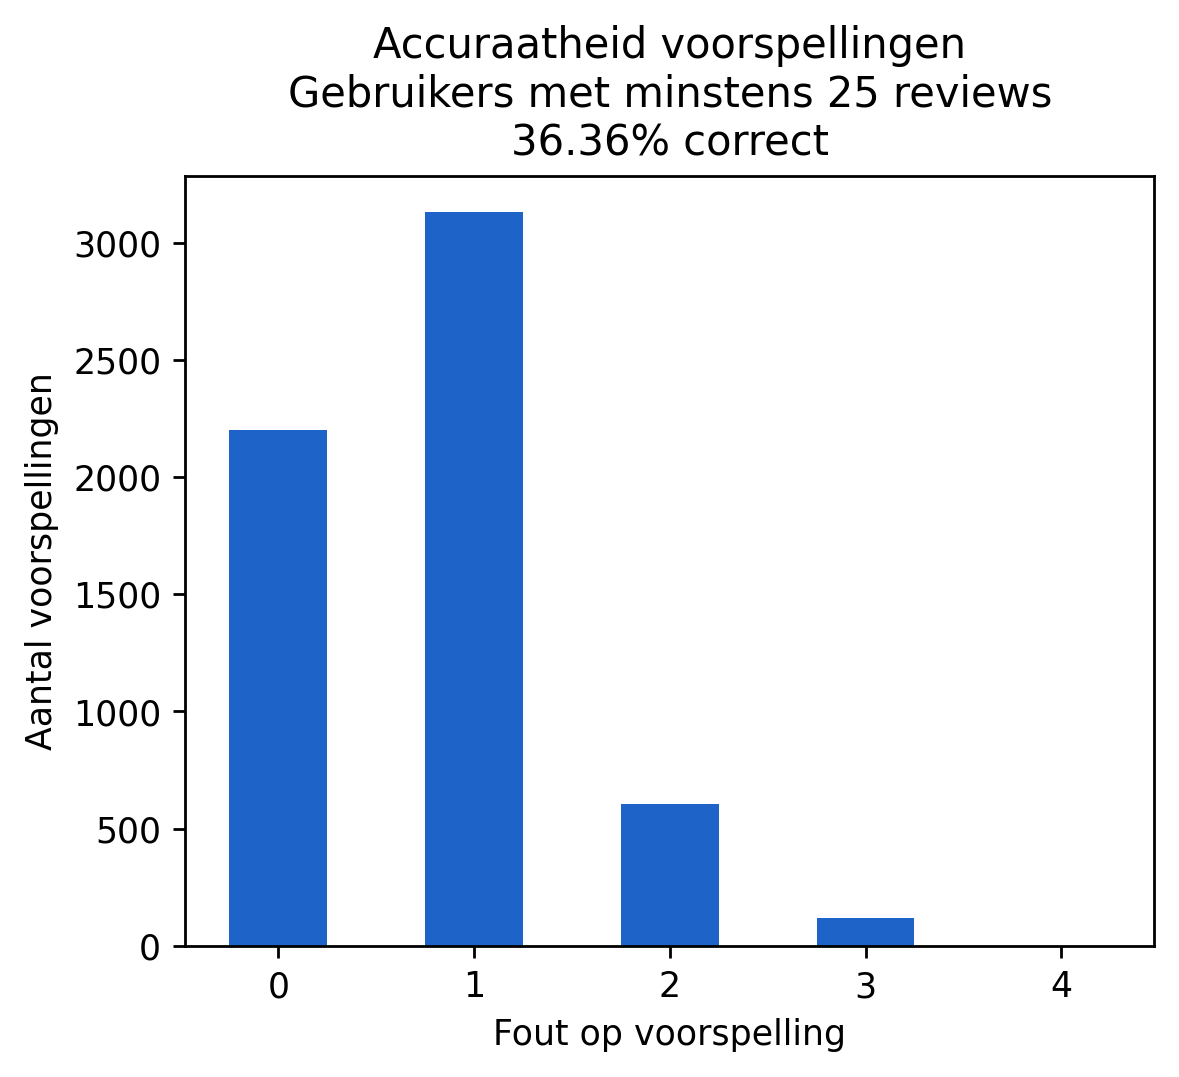
\includegraphics[width=1\linewidth]{fig/chapt5/predictor/accuracy_25+.png}
    \end{subfigure}
    \caption{Accuraatheid voor gebruikers met maximaal vijf reviews versus gebruikers met minimaal 25 reviews}
    \label{fig:chapt5_accuracy_coldstart}
\end{figure}

\subsection{Grootte dataset}
% TODO: NADAT we opsplitsen bij users, een deel van de users weggooien bij de train kant (en bijhorende reviews opnieuw uitrekenen via join), zal ook sneller trainen dan


\subsection{Lossfuncties}
% TODO: lossfuncties heeft ook weinig effect

\subsection{Extreme voorspellingen}
% TODO: analyse van hoe correct we zijn over actual 5-sterren restaurants, en over actual 1-ster-restaurants, daar deze vaak de belangrijkste zijn om juist te hebben. 




\section{Vergelijking met andere methoden}
% TODO: DeepCoNN, traditionele methoden, oof dat gaat veel werk zijn.
% TODO: Bias recommender, die presteert best goed. Maar miss met de accuracy dat we kunnen weerleggen dat goede MSE miss niet altijd overeenkomt met accuracy?
% TODO: zeggen dat onze resultaten in lijn liggen met andere papers/verslagen online
% TODO: random forest werkt ok, als we explainability belangrijk zouden vinden. RMSE van 1.2

\section{Aanbevelingen maken}
% TODO: meerdere mogelijkheden, maar miss out of scope?

\subsection{Diversiteit}



% TODO: apart hoofdstuk voor discussie? Te bespreken
% TODO: bespreek ook de facetten van implemenatie in een reele omgeving, dus dat online algoritme goed is voor nieuwe data, dat het trainen van het neuraal netwerk niet steeds opnieuw hoeft te gebeuren daar het ook goed presteert op kleinere datasets (of niet?), ...
